
	\section{Introduction}
	\label{sec:intro}
	
    %Broad intro
    In 1970, \cite{davis1970clustering} discovered that transitivity---the tendency of friends of friends to be friends themselves---is a prevalent feature in social networks.
    Since that early discovery, real-world networks have been observed to have many other common macroscopic features, and these discoveries have led to probabilistic models for networks that display these phenomena.
    The observation that transitivity and other common subgraphs are prevalent in networks motivated the exponential random graph model (ERGM) \cite{frank1986markov}.
    \cite{barabasi1999emergence} demonstrated that many large networks display a scale-free power law degree distribution, and provided a model for constructing such graphs.
    Similarly, the small world phenomenon---that networks display surprisingly few degrees of separation---motivated the network model in \cite{watts1998collective}.
    While network science is often driven by the observation and modelling of common properties in networks, it is incumbent on the practicing data scientist to explore network data using statistical methods. 
    
    One approach to understanding network data is to fit free parameters in these network models to the data through likelihood-based or Bayesian methods. 
    In \cite{wasserman1996logit}, a pseudolikelihood method was used with graphlet counts to fit an ERGM designed to display transitivity, and Monte Carlo Markov Chain (MCMC) methods were developed in \cite{snijders2002markov} for fitting general ERGMs.
	Fitting such models from data can be cumbersome, and to do so implicitly assumes that the network follows such a model exactly.
	Network statistics, such as the clustering coefficient, algebraic connectivity, and degree sequence, are more flexible tools.
	A good statistic can be used to fit and test models, for example, \cite{watts1998collective} used the local clustering coefficient, a measure of the number of triangles relative to wedges, to test if a network is a small-world graph.
	The clustering coefficient is also used to understand social network graphs, \cite{chakrabarti2006graph}.
	More generally, it was discovered that re-occurring subgraph patterns can be used to differentiate real-world networks, and that genetic networks, neural networks, and internet networks all presented different common interconnectivity patterns, \cite{milo2002network}.
	In this work, we will propose a new method for counting the occurrences of any subgraph pattern, otherwise known as {\em graphlets}---a term coined in \cite{prvzulj2004modeling}---or motifs.
	
\begin{figure}[th]
\begin{center}
\hspace*{\fill}
\minipage{0.06\textwidth}
  
\includegraphics[width=\linewidth]{graphlet_2-1.png}\vspace{-.3cm}
  \caption*{$H_1^{(2)}$}
\endminipage\hfill
\minipage{0.06\textwidth}
  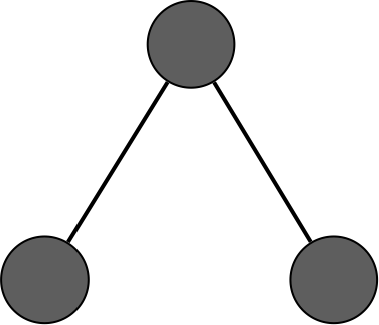
\includegraphics[width=\linewidth]{graphlet_3-1.png}\vspace{-.3cm}
  \caption*{$H_1^{(3)}$}
\endminipage\hfill
\minipage{0.06\textwidth}
  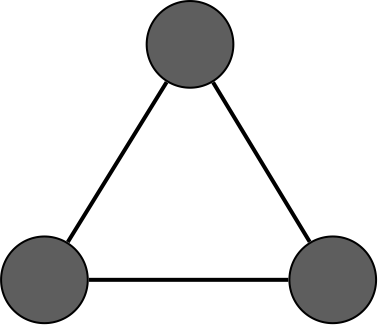
\includegraphics[width=\linewidth]{graphlet_3-2.png}\vspace{-.3cm}
  \caption*{$H_2^{(3)}$}
\endminipage
\hspace*{\fill}
\vskip 5pt
\hspace*{\fill}
\minipage{0.06\textwidth}%
  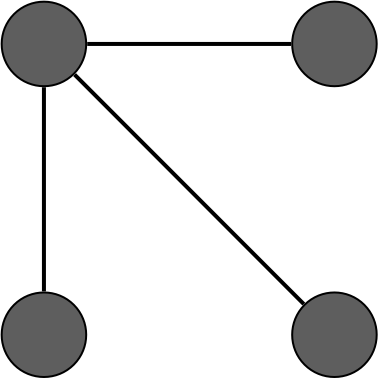
\includegraphics[width=\linewidth]{graphlet_4-1.png}\vspace{-.3cm}
  \caption*{$H_1^{(4)}$}
\endminipage\hfill
\minipage{0.06\textwidth}
  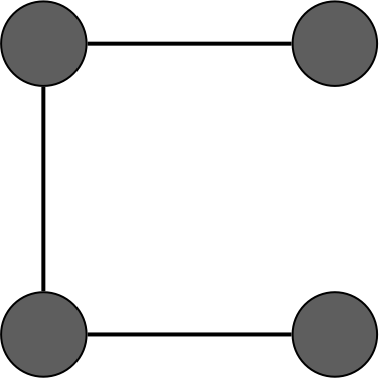
\includegraphics[width=\linewidth]{graphlet_4-2.png}\vspace{-.3cm}
  \caption*{$H_2^{(4)}$}
\endminipage\hfill
\minipage{0.06\textwidth}
  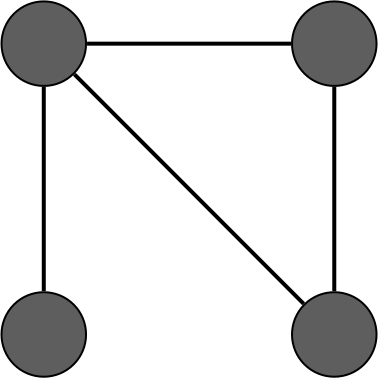
\includegraphics[width=\linewidth]{graphlet_4-3.png}\vspace{-.3cm}
  \caption*{$H_3^{(4)}$}
\endminipage\hfill
\minipage{0.06\textwidth}
  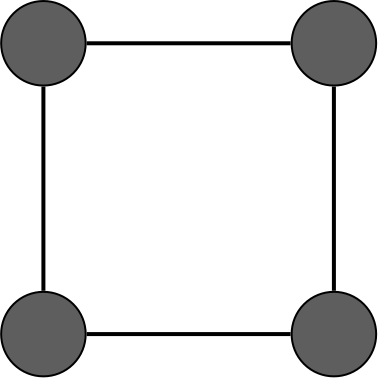
\includegraphics[width=\linewidth]{graphlet_4-4.png}\vspace{-.3cm}
  \caption*{$H_4^{(4)}$}
\endminipage\hfill
\minipage{0.06\textwidth}%
  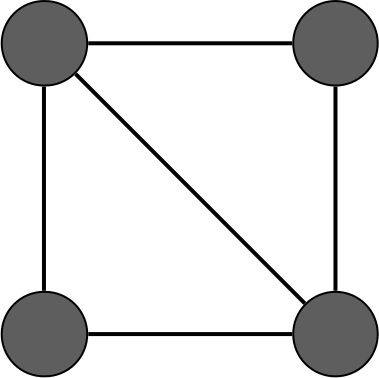
\includegraphics[width=\linewidth]{graphlet_4-5.png}\vspace{-.3cm}
  \caption*{$H_5^{(4)}$}
\endminipage\hspace*{\fill}
\minipage{0.06\textwidth}%
  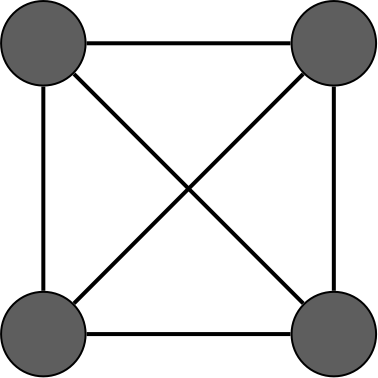
\includegraphics[width=\linewidth]{graphlet_4-6.png}\vspace{-.3cm}
  \caption*{$H_6^{(4)}$}
\endminipage
\hspace*{\fill}
\vskip 5pt
\hspace*{\fill}
\minipage{0.08\textwidth}%
  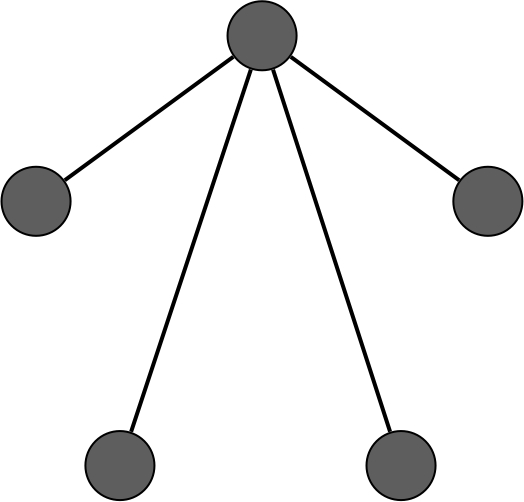
\includegraphics[width=\linewidth]{graphlet_5-1.png}\vspace{-.3cm}
  \caption*{$H_1^{(5)}$}
\endminipage\hfill
\minipage{0.08\textwidth}
  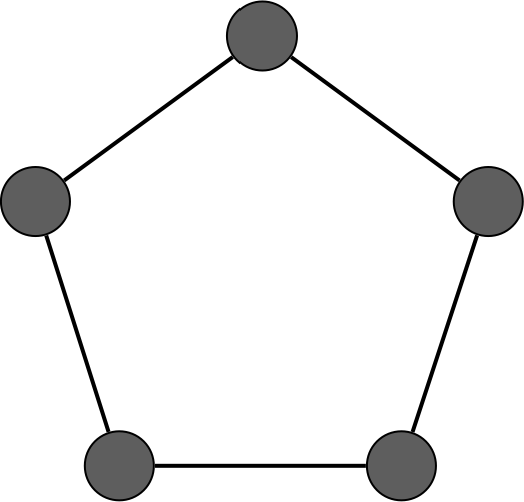
\includegraphics[width=\linewidth]{graphlet_5-8.png}\vspace{-.3cm}
  \caption*{$H_8^{(5)}$}
\endminipage\hfill
\minipage{0.08\textwidth}
  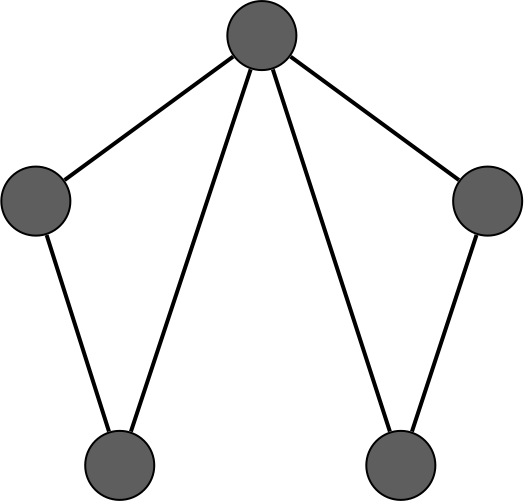
\includegraphics[width=\linewidth]{graphlet_5-11.png}\vspace{-.3cm}
  \caption*{$H_{11}^{(5)}$}
\endminipage\hfill
\minipage{0.08\textwidth}
  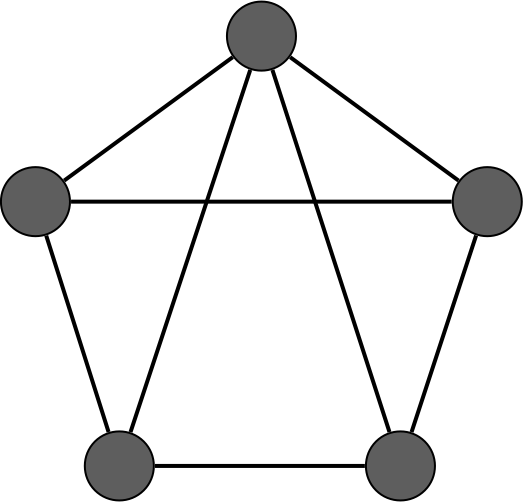
\includegraphics[width=\linewidth]{graphlet_5-19.png}\vspace{-.3cm}
  \caption*{$H_{19}^{(5)}$}
\endminipage\hfill
\minipage{0.08\textwidth}%
  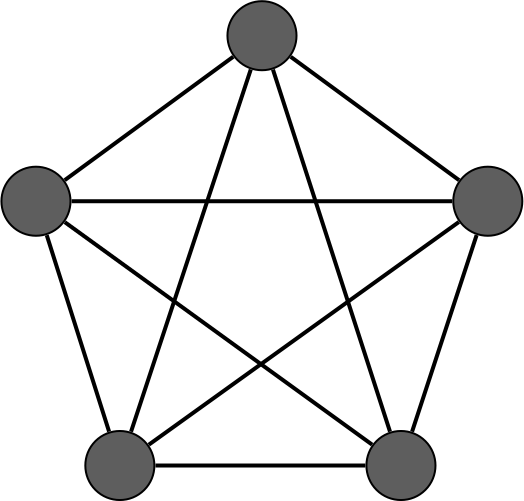
\includegraphics[width=\linewidth]{graphlet_5-21.png}\vspace{-.3cm}
  \caption*{$H_{21}^{(5)}$}
\endminipage\hspace*{\fill}
\vspace{-.1cm}
\caption{Examples of graphlets}
\vspace{-.1cm}
\label{fig:graphlets}
\end{center}
\end{figure}

	
	%Intro to graphlets
	A graphlet is a small connected graph topology, such as a triangle, wedge, or $k$-clique, which we will use to describe the local behavior of a larger network (example graphlets of size 3, 4, and 5, can be seen in Figure \ref{fig:graphlets}).
	Let the graph in question be $G = (V,E)$ where $V$ is a set of vertices and $E$ is a set of unordered pairs of vertices ($G$ is assumed to be undirected and unweighted).
	Imagine specifying a $k$-graphlet and testing for every induced subgraph of the graph (denoted $G|\{v_1,\ldots,v_k\}$ where $v_1,\ldots,v_k \in V$), if it is isomorphic to the subgraph (it has the same topology).
	We would like to compute the number of Connected Induced Subgraphs of size $k$ (denoted by {\em $k$-CIS} throughout) for which this match holds.
	We call this number the {\em graphlet counts} and the proportion of the number of such matches to the total number of $k$-CISs is called the {\em graphlet coefficient}.
	
    Graphlets are the graph analogue of wavelets (small oscillatory functions that are convolved with a signal to produce wavelet coefficients) because they are small topologies that are matched to induced subgraphs of the original graph to produce the graphlet coefficients.
	Graphlet coefficients, also referred to as graph moments, are used in the method of moments to fit certain graph models by selecting parameters that match the empirical graph moments to their expectations \cite{bickel2011method}.
	Graphlet coefficients are used to understand biological networks, such as the protein-protein interaction network, and reoccuring patterns are thought to indicate evolutionary conserved modules \cite{prvzulj2006efficient}. 
	If the graphlet size, $k$, is small then testing for isomorphism, a problem called graph matching \cite{cordella2004sub}, is feasible, but testing every induced subgraph can require on the order of $n^k$ iterations in its most naive implementation.
	We propose a class of methods called lifting that allow us to quickly estimate graphlet coefficients.

	%Graphlet sampling
	
	While there exist several algorithms that can estimate the proportion of triangles, wedges, and graphlets with four or five vertices (for example, \cite{Ahmed2017count, rahman2014graft}), there are few algorithms that can efficiently estimate the proportion of larger graphlets.
	Many methods that can handle arbitrary graphlets are Monte Carlo sampling procedures that traverse through the space of all graphlets of a certain size within the large network.
	Two such methods are GUISE algorithm of \cite{bhuiyan2012guise} and the pairwise subgraph random walk of \cite{Wang2014psrw}, which differ in the way that they perform a random walk between the CIS samples.
	Another option is to generate a sequence of vertices that induces a CIS sample, which has been done in \cite{Han2016waddling} using an algorithm called Waddling random walk.
	Alternatives to random Monte Carlo schemes include the color coding scheme of \cite{Bressan2017colourcoding}, but it processes the whole graph, while the Monte Carlo schemes can traverse the network locally.
    In this work, we propose a new Monte Carlo algorithm, called lifting, for estimating the graphlet counts within a large network.
    The lifting step takes a smaller CIS of size $k-1$ and produces a subgraph of size $k$ by adding an adjacent vertex to it (according to a specific scheme).  
    In this paper we consider procedures that start from vertices or edges and lift to sample CIS of size $k$.
	Lifting is a simple, flexible procedure that can be easily distributed to accommodate massive network datasets.
	
	\subsection{Our contributions}
	
	Graphlet coefficients are multipurpose statistical tools that can be used for model fitting and testing, network regression, and exploratory analysis for network data.
    Any CIS Monte Carlo sampling scheme has three goals: that it provides unbiased estimates of the graphlet coefficients, that the variance of the estimated coefficients is small, and that it does so in as few iterations as possible.
    Because massive graphs are often stored in distributed databases, we would like the sampling scheme to require only neighborhood queries (requests to the database returns the neighbors of a node) and we will avoid storing or processing the full graph.
    Because communication is often the bottleneck in distributed computing, neighborhood queries are the basic unit for measuring computational time complexity.
    
    After discussing the precise requirements for any CIS sampling procedure, we will introduce the lifting scheme for subgraphs.
    The key difficulty in any Monte Carlo method for graphlet counting is calculating the sampling distribution.
    We provide two methods, the ordered lift estimator and the unordered lift estimator, which differ in the way that subgraphs are represented and counted in the graphlet count.
    The ordered estimator allows for a modification, called {\em shotgun sampling} that samples multiple subgraphs in one shot. 
    For our theoretical component, we prove that the estimated graphlet coefficients are unbiased when the underlying MCMC has reached the stationary distribution (called perfect mixing).
    We also prove that under perfect mixing, the variance of the estimator scales like $\Delta^{k-2}$ where $\Delta$ is the maximum degree, and show that the lifting scheme can have significantly lower sample correlations than the subgraph random walk.
    All proofs can be found in the supplement.
    We conclude with real-world network experiments that reinforce the contention that subgraph lifting has a lower variance than Waddling and lower sample correlation than subgraph random walks.

	\section{Sampling graphlets}

	\subsection{Definitions and notation}
	
%	Consider a graph $G=(V,E)$ with set of vertices $V$ and set of edges $E \subseteq \binom{V}{2}$. 
	Throughout we will assume that our graph $G = (V,E)$ is simple, connected and undirected. 
	%(It's easy to translate our results to the case of directed graphs, since we will mostly be focusing on the sampling procedure.) 
	For a subset $W \subseteq V$, a subgraph of $G$ induced by $W$, $G|W$ is a graph with vertices in $W$ and edges in $\binom{W}{2}\cap E$. 
	We call a connected motif on $k$ vertices a $k$-graphlet.
    Given a $k$-graphlet $H$, we'll be interested in the number of $k$-subgraphs of $G$ isomorphic to $H$.
    %In order to distinguish between the abstract graph topology $H$ and the graphlets found in the graph $G$, we will call $H$ a motif, and if the graphlet $T := G|W \sim H$ then it is said to have motif $H$.
	%The distinction between a graphlet and a subgraph is the fact that the subgraph retains the vertex labels, $W$, and the graphlet is only the topology of $G|W$.
	The set of all connected induced $k$-subgraphs (or $k$-CISs) of $G$ is denoted by $\cV_k(G)$ (or simply $\cV_k$).
	
	An unordered set of vertices is denoted $\{v_1,\ldots,v_k\}$ while an ordered list is denoted $[v_1,\ldots,v_k]$.
	Let $H_1, H_2, \ldots, H_l$ be all non-isomorphic
	motifs for which we would like the graphlet counts. 
	For $T\in \cV_k(G)$, we say that ``$T$ is subgraph of
	 type $m$'' if $T$ is isomorphic to $H_m$, and denote this with $T \sim H_m$.
	The number of $k$-subgraphs in $G$ of type $m$ is equal to 
	$N_m (G) = \sum_{T \in \cV_k(G)} \ind(T \sim H_m)$, where $\ind(A)$ 
	is the indicator function.
    For a subgraph $S \subseteq G$, denote $V_S$ to be the set of its vertices, $E_S$ to be the set of its edges.
	Denote $\cN_v(S)$ (vertex neighborhood of $S$) to be the set of all vertices adjacent to some vertex in $S$ not including $S$ itself. 
	Denote $\cN_e(S)$ (edge neighborhood of $S$) to be the set of all edges that connect a vertex from $S$ and a vertex outside of $S$.
% 	Formally,
% 	\begin{equation*}
% 		\cN_v(S) = \{u\in V_G\setminus V_S \mid \exists s\in V_S : (s,u)\in E_G\},
% 	\end{equation*}
% 	\begin{equation*}
% 		\cN_e(S) = \{(s,u)\in E_G \mid s\in V_S, u\notin V_S\}.
% 	\end{equation*}	
	Also, denote $\deg(S)$ (degree of $S$) to be the number of edges in $\cN_e(S)$, and denote $\deg_S(u)$ ($S$-degree of $u$) to be the number of vertices from $S$ that are connected to $u$.
% 	Formally,
% 	\begin{equation*}
% 		\deg(S) = |\{(s,u)\in E_G \mid s\in V_S, u\notin V_S\}|,
% 	\end{equation*}
% 	\begin{equation*}
% 		\deg_S(u) = |\{s\in V_S\mid (u,s)\in E_G\}|.
% 	\end{equation*}
	Note that $\deg(S) + 2|E_S| = \sum_{v\in V_S} \deg(v)$.


    \subsection{Prior graphlet sampling methods}
	
The ideal Monte Carlo procedure would sequentially sample CISs uniformly at random from the set $\cV_k(G)$, classify their type, and update the corresponding counts.  
Unfortunately, uniformly sampling CISs is not a simple task because they are required to be connected---a random set of k vertices is unlikely to be connected.
CIS sampling methods require Monte Carlo Markov Chains (MCMCs) for which one can calculate the stationary distribution, $\pi$, over the elements of $\cV_k$.
First, let us consider how we update the graphlet counts, $N_m(G)$, given a sample of CISs, $T_1, T_2, \ldots, T_n$.

The desire to sample subgraphs uniformly is natural, because the empirical counts will be unbiased estimates of their population quantities.
Instead, suppose that our CIS sample, with $T_i \in \cV_k, i=1,\ldots,n$, is drawn with known sampling distribution $\pi$.
Then we use Horvitz-Thompson inverse probability weighting to estimate the graphlet counts,
\begin{equation}
  \label{eq:moments}
  \hat N_m(G) := \frac{1}{n} \sum_{i=1}^n \frac{\ind(T_i\sim H_m)}{\pi(T_i)}.  
\end{equation}
It is simple to see that this is an unbiased estimate of the graphlet counts as long as $\pi$ is supported over all elements of $\cV_k$.
Alternative updating methods include rejection sampling, which can be combined with inverse probability weighting, but we will use \eqref{eq:moments} for ease of presentation.

We find ourselves in a game, where we can choose any CIS Monte Carlo algorithm that induces a stationary distribution $\pi$, but we must be able to quickly and accurately compute $\pi$ in order to use \eqref{eq:moments}.
We will analyze the theoretical implications of the sampling algorithm based on mixing times of the Markov chain and the variance of the graphlet count estimates.
Before we explore the lifting procedure, this paper's algorithmic contribution, we would like to discuss some existing MCMC CIS sampling methods.

%\subsection{Subgraph random walks}

%Any admissible graphlet Markov chain transitions between k-graphlets of $G$ and the transition probabilities have a calculable stationary distribution $\pi$.
% The basic algorithm is listed in \ref{alg:SRW}, and some elements are left purposefully vague to maintain generality.
% Many of the proposed graphlet sampling algorithms can be encompassed by this master algorithm, and we will highlight the two most prominent examples: Subgraph random walk and waddling random walk.

% \begin{algorithm}
% \label{alg:SMC}
% \caption{Subgraph Markov chain}
% \begin{algorithmic}
%   \STATE Initialize $T$ at an arbitrary k-graphlet, $n \gets 1$, $\hat N_m(G) \gets 0$
%   \WHILE{stopping criteria is not met}
%   \STATE Query the neighbors of each vertex in $T$, $\{\mathcal N (v): v \in T\}$
%   \STATE Add a vertex according to an {\em add rule}
%   \STATE Remove a vertex according to a {\em remove rule}
%   \IF{{\em Markov chain is sufficiently mixed}}
%   \STATE Determine the type $m$ of $T$, calculate $\pi(T)$
%   \STATE Update $\hat N_m(G) \gets ((n -1) \hat N_m(G) + \pi^{-1}(T))/n$ and $n \gets n + 1$
%   \ENDIF
%   \ENDWHILE
% \end{algorithmic}
% \end{algorithm}


The subgraph random walk is described in \cite{Wang2014psrw}, where they make a modification called the pairwise subgraph random walk (PSRW).
%For this method, consider a set $\_k$ of all $k$-graphlets of $G$.
In order to perform a random walk where the states are $\cV_k$, we form the CIS-relationship graph.
Two $k$-CISs, $T,S \in \cV_k$ are connected with an edge if and only if vertex sets of $T$ and $S$ differ by one element, i.e. when $|V(T) \cap V(S)| = k-1$.
Given the graph structure, we sample $k$-CISs by a random walk on the set $\cV_k$, which is called Subgraph Random Walk (SRW).
Because the transition from state $S \in \cV_k$ is made uniformly at random to each adjacent CIS, then we know that the stationary distribution will sample each edge in the CIS-relationship graph with equal probability.
This fact enables \cite{Wang2014psrw} to provide a local estimator of the stationary probability $\pi(S)$.
PSRW is a modification of the SRW algorithm, where each transition is performed from $S$ to $T$ in $\cV_{k-1}$ and then the $k$-CIS $S \cup T$ is returned.
	%This is the basic lift operation, and it was used in the PSRW algorithm, \cite{Wang2014psrw}, to generate $k$-graphlets from a subgraph random walk on $k-1$-subgraphs.

The mixing time is a critical issue for any MCMC, and subgraph sampling is no exception.
Dependence between consecutive samples results in a higher variability of $\hat N_m(G)$, and sufficient mixing is required for the stationary distribution to approximate the sampling distribution.
It was pointed out in \cite{Bressan2017colourcoding} that the mixing time of the SRW can be of order $O(n^{k-2})$, even if the mixing time of the random walk on the original graph $G$ is of constant order $O(1)$.
PSRW also requires global constants based on the CIS-graph, which can be computationally intractable (super-linear time).

Another approach is to sample on ordered sequences of vertices $[v_1, \ldots, v_k]$, denoted by $A$, which would induce a $k$-CIS, $T = G|A$.
Given a sampling scheme of such sequences with probability $\tilde\pi(A)$, the estimator for graphlet counts is given by
\begin{equation}
  \label{eq:sequences}
  \hat N_m(G) := \frac{\omega_m}{n} \sum_{i=1}^n \frac{\ind(G|A_i\sim H_m)}{\tilde\pi(A_i)}
\end{equation}
for some fixed weights $\omega_m$.  
The main difference between these types of sampling is that we maintain the ordering of the vertices, while a CIS is an unordered set of vertices.

A naive method for sampling such sequences would be to perform a random walk on the graph $G$ and then sample the $k$ vertices most recently visited.
This scheme is appealing because it has an easy to compute stationary distribution, and can `inherit' the mixing rate from the random walk on $G$ (which is relatively small).
Despite these advantages, certain graphlet topologies, such as stars, will never be sampled, and modifications are needed to remedy this defect.
\cite{chen2016general} combined this basic idea with the SRW by maintaining a $l$ length history of the SRW on CISs of size $k-l+1$, and unioning the history, but this suffers from the same issues as SRW, such as slow mixing and the need to calculate global constants based on the CIS-graph.

\cite{Han2016waddling} introduced a {\em Waddling} protocol which retains a memory of the last $s$ vertices in the random walk on $G$ and then extends this subgraph by $k-s$ vertices from either the first or last vertex visited in the $s$-subgraph (this extension is known as the `waddle').
The authors provide a method for calculating the stationary distribution for this MCMC, and prove a bound on the error for the graphlet coefficients.
The downside to this method is that the precise Waddling protocol used should depend on the desired graphlet, and the algorithm involves a rejection step which may lead to a loss of efficiency.
In contrast, the lifting scheme has the advantage of inheriting the mixing time of the random walk on $G$, and it can simultaneously sample many CISs of differing sizes without any rejections.


% \subsection{Lifting procedures}

%     This approach gives an unbiased estimator assuming $\pi_k(T) >0$ for any $T\in \cV_k$.
%     The biggest issue of this method is the variance of $\hat N_m(G)$. We rewrite the variance as a sum of two terms:
% 	\begin{multline}
% 	\label{eq:variation}
% 		\Var(\hat N_m(G)) = \frac{1}{n}\left( \E_{\pi_k} \frac{\ind(T\sim H_m)}{\pi_k(T)^2} - N_m^2(G)\right) +\\
% 		\frac{2}{n^2} \sum_{i < j} \Cov_{\pi_k}\left( \frac{\ind(T_i\sim H_m)}{\pi_k(T_i)}, \frac{\ind(T_j\sim H_m)}{\pi_k(T_j)}\right).
% 	\end{multline}
	
% 	The first term will be referred to as variation under independence term, and can dominate the sum if $\pi_k(T)$ greatly deviates from the uniform probability $\rho(T) = \frac{\ind(T\sim H_m)}{N_m(G)}$.
% 	The second term will be referred to as a covariance term and can dominate the sum when graphlets $T_i$ and $T_{i+1}$ have high correlation, which is the case for Subgraph Random Walk methods discussed below.
	
% 	The previous papers on that topic focused on efficient method of sampling a sequence of $k$-graphlets, depending on a framework.
% 	We'll try to summarize the frameworks and corresponding methods here.
	
% 	There are two different frameworks, each with its own problem statement.
% 	\begin{itemize}
% 		\item \textbf{Framework 1.} We have access to the whole graph structure, for example, in the form of adjacency matrix. 
% 		We can sample the nodes of the graph cheaply, independently and according to an arbitrary probability distribution.
% 		The goal is to sample graphlets quickly, uniformly and independently.
% 		In particular, the covariance term would be irrelevant in this framework.
% 		The state-of-art method for this framework is Color Coding \cite{Bressan2017colourcoding}.

% 		\item \textbf{Framework 2.} We start with an access to a single node $v_0$ and its 
% 		neighborhood. As a query, we can transition to a neighboring node $v_1$ and get access to the neighborhood of $v_1$.
% 		Each moment of time we can only get access to the neighbors of previously visited nodes. 
% 		This framework is applied when queries are either expensive or limited and traversing the whole graph is time-prohibitive at best and not feasible at worst. 
% 		The goal here is to achieve best accuracy with either limited number of queries ($10^3-10^4$ queries for graphs with $10^5-10^6$ nodes) or limited time, or something in between (costly queries).
% 		Recent methods include Subgraph Random Walk(SRW) and Pairwise Random Walk \cite{Wang2014psrw} and Waddling Random Walk (WRW) \cite{Han2016waddling}.
% 	\end{itemize}
	
% 	For each of the two frameworks above we'll present a modification of the base algorithm
% 	to suit corresponding goals.
	
% 	\subsection{Subgraph Random Walk (SRW)}
	

% 	For a subgraph $S \subseteq G$, denote $V_S$ to be the set of its vertices, $E_S$ to be the set of its edges.
% 	Denote $\cN_v(S)$ (vertex neighborhood of $S$) to be the set of all vertices adjacent to some vertex in $S$ not including $S$ itself. 
% 	Denote $\cN_e(S)$ (edge neighborhood of $S$) to be the set of all edges that connect a vertex from $S$ and a vertex outside of $S$.
% 	Formally,
% 	\begin{equation*}
% 		\cN_v(S) = \{u\in V_G\setminus V_S \mid \exists s\in V_S : (s,u)\in E_G\},
% 	\end{equation*}
% 	\begin{equation*}
% 		\cN_e(S) = \{(s,u)\in E_G \mid s\in V_S, u\notin V_S\}.
% 	\end{equation*}	
	
% 	Denote $\deg(S)$ (degree of $S$) to be the number of edges in $\cN_e(S)$, and denote $\deg_S(u)$ ($S$-degree of $u$) to be the number of vertices from $S$ that are connected to $u$.
% 	Formally,
% 	\begin{equation*}
% 		\deg(S) = |\{(s,u)\in E_G \mid s\in V_S, u\notin V_S\}|,
% 	\end{equation*}
% 	\begin{equation*}
% 		\deg_S(u) = |\{s\in V_S\mid (u,s)\in E_G\}|.
% 	\end{equation*}
% 	Note that $\deg(S) + 2|E_S| = \sum_{v\in V_S} \deg(v)$.

\section{Subgraph lifting}
	
	The lifting algorithm is based on a randomized protocol of attaching a vertex to a given CIS.
	For any \smash{$(k-1)$}-CIS, $S$ we lift it to a $k$-subgraph by adding a vertex from its neighborhood, $\cN_v(S)$ at random according to some probability distribution.
	Note that this basic lifting operation can explore any possible subgraph in $\cV_k$. 
	%Another way to think about the lift operation is to perform a transition of the SRW, from $S$ to $T$ in $\cV_{k-1}$ and then returning $S \cup T$.
	%This is the basic lift operation, and it was used in the PSRW algorithm, \cite{Wang2014psrw}, to generate $k$-graphlets from a subgraph random walk on $k-1$-subgraphs.
	In this work, we show that one can lift from a random walk on the vertices, or another vertex or edge sampling distribution, and achieve favorable properties.
	

\begin{figure}[th]
\begin{center}
\hspace*{\fill}
\minipage{0.10\textwidth}
  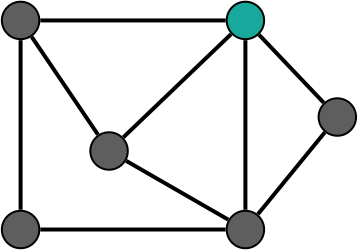
\includegraphics[width=\linewidth]{lift_1.png}
  \caption*{(a)}
\endminipage\hfill
\minipage{0.10\textwidth}
  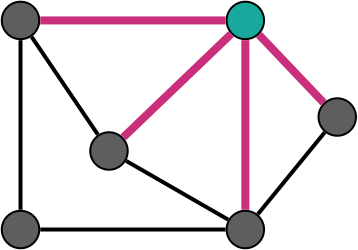
\includegraphics[width=\linewidth]{lift_2.png}
  \caption*{(b)}
\endminipage\hfill
\minipage{0.10\textwidth}
  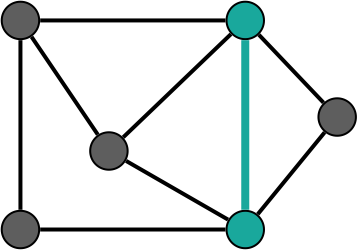
\includegraphics[width=\linewidth]{lift_3.png}
  \caption*{(c)}
\endminipage\hfill
\minipage{0.10\textwidth}%
  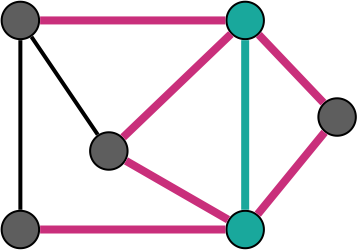
\includegraphics[width=\linewidth]{lift_4.png}
  \caption*{(d)}
\endminipage
\hspace*{\fill}
\vskip 5pt
\hspace*{\fill}
\minipage{0.10\textwidth}
  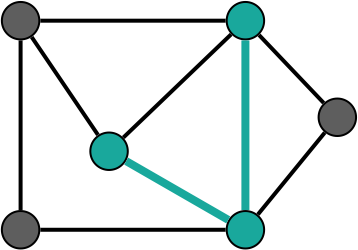
\includegraphics[width=\linewidth]{lift_5.png}
  \caption*{(e)}
\endminipage\hfill
\minipage{0.10\textwidth}
  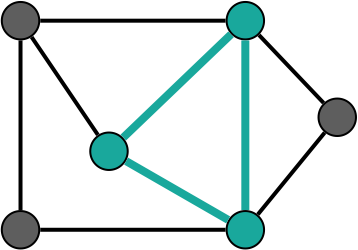
\includegraphics[width=\linewidth]{lift_6.png}
  \caption*{(f)}
\endminipage\hfill
\minipage{0.10\textwidth}
  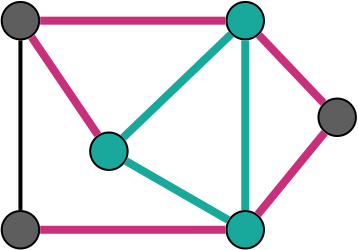
\includegraphics[width=\linewidth]{lift_7.png}
  \caption*{(g)}
\endminipage\hfill
\minipage{0.10\textwidth}%
  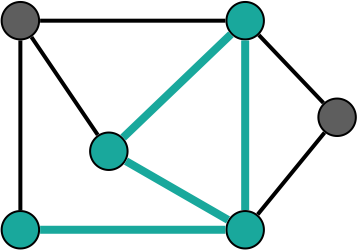
\includegraphics[width=\linewidth]{lift_8.png}
  \caption*{(h)}
\endminipage\hspace*{\fill}
\caption{Lifting procedure}
\label{fig:lifting}
\end{center}
\end{figure}

    You can see an example of the lifting sampling scheme in Figure \ref{fig:lifting}, where the algorithm iteratively builds a $4$-CIS from a chosen node.
	%The lifting sampling scheme iteratively builds larger subgraphs from smaller ones, and you can see an example in Figure \ref{fig:lifting}.
	First assume we have a node $v_1$ sampled from the distribution $\pi_1$, a base distribution that can be computed from local information (step (a)). 
	We assume that $\pi_1(v) = \frac{f(\deg(v))}{K}$, where $f(x)$ is some function (usually a polynomial) and $K$ is some global normalizing constant which is assumed to be precomputed.
	Denote $S_1 = \{v_1\}$.
    To start our procedure, sample an edge $(v_1,v_2)$ uniformly from $\cN_e(S_1)$ (step (b)). 
	The vertex $v_2$ is then attached to $S_1$, forming a subgraph $S_2 = G|(V_{S_1} + {v_2})$ (step (c)).
	After that, we sample another edge $(v_i, v_3)$ (with $1\leq i\leq 2$) uniformly from $\cN_e(S_2)$, and the vertex $v_3$ is then attached to $S_2$ (steps (d-f)).
	At each step we sample an edge $(v_i, v_{r+1})$ (with $1\leq i \leq r$) from $\cN_e(S_r)$ uniformly at random, and attach the vertex $v_{r+1}$ to the subgraph $S_r$ (steps (g-h)).
	After $k-1$ operations, we obtain a $k$-CIS $T = S_k$.
	We'll refer to the procedure above as the {\em lifting procedure starting at vertex $v_1$}.

    By induction, we can see that every $k$-CIS has a non-zero probability of being visited, assuming that $\pi_1$ is supported on every vertex.
	The Waddling method was motivated by the fact that a simple random walk would not visit all subgraphs in $\cV_k$, yet Waddling only partially solved this issue, because not every wadding protocol can sample every $k$-graphlet.
    Typically, $\pi_1$ is assumed to be the stationary distribution of a simple random walk, but it could be another distribution such as uniform sampling over the vertices or edges.
	One motivation for lifting is that if we sample the vertices from a simple random walk, then lifting `inherits' its mixing time, much like Waddling.
	Hence, lifting is a simple algorithm that can sample any CIS with good mixing rates and no rejections.
	It remains to be demonstrated that we can calculate the probability of sampling the $k$-CIS $\pi(S)$ using only local information.
	
	\subsection{Ordered lift estimator}
	
	%When we sample a $k$-CIS, we match this to a $k$-graphlet through a graph isomorphism algorithm.
	%Alternatively, we can maintain an ordering of the vertices, and count {\em ordered $k$-CISs}, which is are $k$-CISs where the vertices are labelled from $1,\ldots,k$.
 %   Then at the end of the algorithm we combine the ordered $k$-graphlet counts that correspond to the same topology.
    
    We can think of a lifting procedure as a way of sampling a sequence $A = [v_1, \ldots, v_k]$, ordered from the first vertex sampled to the last, that is then used to generate a CIS.
	Denote the set of such sequences as $V^k_G$.
%	For $A = [v_1, \ldots, v_k] \in V^k_G$, denote $A[i]:=v_i$.
	Let $S_r = G|\{v_1,\ldots, v_r\}$ be the $r$-CIS obtained by the lifting procedure on step $r$.
	The probability of sampling vertex $v_{r+1}$ on the step $r+1$ is equal to
	\begin{equation*}
	    \mathbb{P}(v_{r+1}|S_{r}) := \frac{\deg_{S_r}(v_{r+1})}{|\cN_e(S_r)|} =
	    \frac{|E_{S_{r+1}}| - |E_{S_r}|}{\sum_{i=1}^r \deg(v_i) - 2|E_{S_r}|}.
	\end{equation*}
	Thus, the probability of sampling a sequence $A \in V^k_G$ is equal to
	\begin{multline}
	\label{eq:tildepi}
	    \Tilde\pi(A) := \pi_1(v_1)\prod_{r=1}^{k-1} \P\left(v_{r+1}|S_r\right) =\\
	    \frac{f(\deg(v_1))}{K} \prod_{r=1}^{k-1} \frac{|E_{S_{r+1}}| - |E_{S_r}|}{\sum_{i=1}^r \deg(v_i) - 2|E_{S_r}|}.
	\end{multline}
    Critically, this equation can be computed with only neighborhood information about the involved vertices, so it takes $O(k)$ neighborhood queries.
    Because there are many orderings that could have led to the same CIS $T$, then we need to apply proper weights in the graphlet count estimate \eqref{eq:sequences} by enumerating the number of possible orderings.
    
	Consider the sampled $k$-CIS $T := S_k$.
	Denote the set of possible sequences $A = [v_1,\ldots, v_k]$ that would form $T$ in the lifting process as $\co(T)$.
	Notice that $S_r = G|\{v_1,\ldots,v_r\}$ must be a connected subgraph for all $r$.
	Thus,
	\begin{multline}
	\label{eq:co}
	    \co(T) = \big\{\,[v_1,\ldots,v_k]\in V^k_G \mid \{v_1,\ldots,v_k\} = V_T,\\  T|\{v_1,\ldots,v_r\} \text{ is connected }\big\}.
	\end{multline}
	Since the elements of $\co(T)$ are just certain orderings of vertices in $T$, we call an element from $\co(T)$ a \textit{compatible ordering} of $T$.
	Note that $|\co(T)|$ only depends on the type of the graphlet isomorphic to $T$, and it can be precomputed using dynamic programming.
	Thus, when $T\sim H_m$, the number of compatible orderings are equal: $|\co(H_m)| = |\co(T)|$. Note that $|\co(H_m)|$ can vary from $2^{k-1}$ (for $k$-path) to $k!$ (for $k$-clique).
	We set up the estimator from \eqref{eq:sequences} as
	\begin{equation}
	\label{eq:ord_est}
	    \hat N_{O,m} := \frac{1}{n}\frac{1}{|\co(H_m)|} \sum_{i=1}^n \frac{\ind(G|A_i\sim H_m)}{\tilde\pi(A_i)}.
	\end{equation}
	We call it the {\em ordered lift estimator} for the graphlet count.

\begin{algorithm}[h]
\label{alg:OLE}
\caption{Ordered Lift Estimator (with optional shotgun sampling)}
\begin{algorithmic}
    \INPUT Graph $G$, $k$-graphlet $H_m$
    \OUTPUT $\hat N_m(G)$
    \STATE Count $|\co(H_m)|$- the number of compatible orderings in $H_m$.
    \STATE Initialize $v$ at an arbitrary node, $n \gets 0$, $\hat N_m(G) \gets 0$
    \WHILE{stopping criteria is not met}
        \STATE Sample $v_1$ from $\pi_1(v)$
        \STATE Initialize $V_S \gets \{v_1\}$ and $E_S \gets \{\}$
        \STATE Initialize $\cN_e(S)\gets \cN_e(v_1)$
        \STATE Initialize $\pi(S) \gets \pi_1(v_1)$
        \WHILE{$|V_S| < k-1$}
            \STATE Sample an edge $e=(v,u)$ uniformly from $\cN_e(S)$, with $v\in V_S$ and $u\notin V_S$
            \STATE Set $E_S(u) \gets \{(v,u)\in \cN_e(S)\}$
            \STATE Update $\pi(S)\gets \pi(S)\frac{|E_S(u)|}{|\cN_e(S)|}$
            \STATE Update $V_S\gets V_S\cup\{u\}$ and $E_S \gets E_S \cup E_S(u)$
            \STATE Query $\cN_e(u)$
            \STATE Update $\cN_e(S) \gets [\cN_e(S)\cup\cN_e(u)]\setminus E_S(u)$
        \ENDWHILE
        \IF {not shotgun sampling}
            \STATE Sample an edge $e=(v,u)$ uniformly from $\cN_e(S)$, with $v\in V_S$ and $u\notin V_S$
            \STATE Set $E_S(u) \gets \{(v,u)\in \cN_e(S)\}$
            \STATE Set $\pi(T)\gets \pi(S)\frac{|E_S(u)|}{|\cN_e(S)|}$
            \STATE Set $V_T\gets V_S\cup\{u\}$ and $E_T \gets E_S\cup E_S(u)$
            \IF {$(V_T, E_T) \sim H_m$}
                \STATE Update $\hat N_m(G) \gets \hat N_m(G) + \pi^{-1}(T)$ 
            \ENDIF
        \ENDIF
        \IF {shotgun sampling}
            \FORALL{$u\in \cN_v(S)$}
                \STATE Set $E_S(u) \gets \{(v,u)\in \cN_e(S)\}$
                \STATE Set $V_T\gets V_S\cup\{u\}$ and $E_T \gets E_S \cup E_S(u)$
                \IF{$(V_T, E_T) \sim H_m$}
                    \STATE Update $\hat N_m(G) \gets \hat N_m(G) + \pi^{-1}(S)$
                \ENDIF
            \ENDFOR
        \ENDIF
        \STATE Update $n \gets n + 1$
    \ENDWHILE
    \STATE Normalize $\hat N_m(G) \gets \frac{1}{n}\frac{1}{|\co(H_m)|}\hat N_m(G)$
\end{algorithmic}
\end{algorithm}
	
	A drawback of the algorithm is that it takes $k-1$ queries to lift the CIS plus the number of steps required to sample the first vertex (when sampled from Markov chain). 
	To increase the number of samples per query, notice that if we sample $B = [v_1, \ldots, v_{k-1}]$ via lifting, we can get subgraphs induced by $A = [v_1,\ldots, v_{k-1},u]$ for all $u \in \cN_v(B)$ without any additional queries.
	
	Thus, for each sampled sequence $B_i \in V_G^{k-1}$, we can compute the sum $\sum_{u\in \cN_v(B_i)} \ind(G|B_i \cup \{u\} \sim H_m)$ to incorporate the information about all $k$-CISs in the neighborhood of $B_i$.
	We call this procedure {\em shotgun sampling}.
	The corresponding estimator based on \eqref{eq:sequences} is
	\begin{equation}
	\label{eq:shot_est}
	    \hat N_{S,m} = \frac{1}{n}\frac{1}{|\co(H_m)|} \sum_{i=1}^n \frac{\sum_{u \in \cN_v(B_i)} \ind(G|B_i \cup \{u\} \sim H_m)}{\tilde \pi(B_i)}.
	\end{equation}
	Shotgun sampling produces more CIS samples with no additional query cost, but the CIS samples generated in a single iteration will be highly dependent.
	%independence of CIS samples from two consecutive shotgun shots heavily relies on the well-mixing of sampled sequences $B_i$.
	The following proposition states that the resulting estimators are unbiased.
	
	\begin{proposition}
	\label{prop:unbiased}
    The ordered lifted estimator, $\hat N_{O,m}$, and the shotgun estimator, $\hat N_{S,m}$, are unbiased for the graphlet counts $N_m$.
    \end{proposition}
	
% 	Shotgun sampling is useful in cases when the number of queries is limited, but has a drawback of high correlation between samples.
% 	If the initial vertex $v_1$ was sampled from a random walk, the number of steps between initial vertices should be chosen so that shotgun shots are sufficiently far apart from each other.
	
	\subsection{Unordered lift estimator}
	
	The ordered lift estimators computed the probability of sampling the CIS and the order of included vertices.
	Alternatively, we can compute the marginal probability of sampling the unordered graphlet, $\pi_U(T)$ for the lifted CIS $T \in \cV_k(G)$.
    One advantage of this approach is that this probability is a function of only the degrees of vertices $V_T$.
	%We can also use the estimator \eqref{eq:moments} for the sampling space of $k$-graphlets $\cV_k(G)$.
	%In order to do that, we need to compute the probability $\pi_k(T)$ of getting a particular $k$-graphlet $T \in \cV_k(G)$ in the lifting procedure.
	This can be done either recursively or directly. 
	Throughout, let the set of vertices of $T$ be $v_1,\ldots,v_k$.
	
	We begin the algorithm by querying the probability of obtaining any vertex in $T$, $\pi_1(v_i), i=1,\ldots,k$.
	%As with the Recursive formula starts with known probabilities of initial vertices $\pi_1(v_i)$.
	We will build the probability of obtaining any connected subgraph of $T$ inductively.
	This is possible because the probability of getting $T$ via lifting is given by the sum $\pi_U(T) = \sum_S \mathbb{P}(T|S) \pi_{U}(S)$, where the sum is taken over all connected \smash{$(k-1)$}-subgraphs $S\subset T$, and $\mathbb{P}(T|S)$ denotes the probability of getting from $S$ to $T$ in the lifting procedure.
	%Let $T\setminus S$ be the unique vertex of $T$ that is not in $S$.
	Then
	\begin{multline}
	\label{eq:recursive}
		\pi_{U}(T) = \sum_{S\subset T} \pi_{U}(S) \frac{\deg_S (V_T\setminus V_S)}{|\cN_e(S)|} = \\
		\sum_{S\subset T} \pi_{U}(S) \frac{|E_T| - |E_S|}
		{\sum_{u\in S} \deg(u) - 2|E_S|},
	\end{multline}
	where the sum is taken over all connected \smash{$(k-1)$}-subgraphs $S\subset T$.
	
	For a direct formula, we notice that $\pi_U(T) = \sum_{A\in \co(T)} \tilde\pi(A)$, where $\co(T)$ is the set of compatible orderings of $T$ from previous section, and $\tilde\pi(A)$ is the probability of getting sequence $A\in \co(T)$ in the lifting process (see \eqref{eq:co},\eqref{eq:tildepi}).
	Then 
	\begin{equation}
	\label{eq:direct}
		\pi_U(T) = \sum_{A\in\co(T)} \frac{f(\deg(A[1]))}{K} \prod_{r=1}^{k-1} \frac{|E_{S_{r+1}(A)}| - |E_{S_r(A)}|}{\sum_{i=1}^r \deg(A[i]) - 2|E_{S_r(A)}|},
	\end{equation}
	where, given $A=[v_1,\ldots,v_k]$, $A[i]$ is the $i$th vertex in $A$ and $S_r(A) = G|\{v_1,\ldots,v_r\}$.
	
	Although calculation of this probability on-the-fly is cost-prohibitive, we can greatly reduce the number of operations by noticing that the probability $\pi_k(T)$ is a 
	function of degrees of the vertices: for a CIS $T$ of type $m$, let $[v_1, \ldots, v_k]$ be an arbitrary labelling of the vertices of $T$ with $d_i = \deg(v_i)$, then the probability of $T$ is
	\begin{equation*}
	    \pi_U(T) =\frac{1}{K} F_m(d_1, \ldots, d_k)
	\end{equation*}
    for a cached function $F_m$ given by \eqref{eq:direct}.
	
	\textbf{Example.} Consider a triangle, which is a 3-graphlet with edges $(v_1,v_2)$, 
	$(v_2, v_3)$ and $(v_1,v_3)$. Given the degrees $d_1, d_2, d_3$ of the corresponding 
	vertices, the probability function is
	\begin{multline}
	\label{prob:triangle}
		\pi_U(\mathrm{triangle}) = \left( \frac{\pi_1(d_1)}{d_1} + 
		\frac{\pi_1(d_2)}{d_2}\right) \frac{2}{d_1+d_2-2} +\\ 
		+ \left( \frac{\pi_1(d_2)}{d_2} + \frac{\pi_1(d_3)}{d_3}\right) 
		\frac{2}{d_2+d_3-2} +\\
		\left( \frac{\pi_1(d_3)}{d_3} + \frac{\pi_1(d_1)}{d_1}\right) 
		\frac{2}{d_3+d_1-2}.
	\end{multline}
	
	\textbf{Example.} Consider a wedge, which is a 3-graphlet with edges $(v_1,v_2)$ and 
	$(v_1,v_3)$. Given the degrees $d_1, d_2, d_3$ of the corresponding 
	vertices, the probability function is
	\begin{multline}
	\label{prob:wedge}
		\pi_U(\mathrm{wedge}) = \left( \frac{\pi_1(d_1)}{d_1} + \frac{\pi_1(d_2)}{d_2}\right) \frac{1}{d_1+d_2-2} +\\
		\left( \frac{\pi_1(d_1)}{d_1} + \frac{\pi_1(d_3)}{d_3}\right) \frac{1}{d_1+d_3-2}.
	\end{multline}

	We need to only compute functions $F_m$ once before starting the algorithm.
	When a $k$-CIS $T$ is sampled via lifting procedure, we find the natural labelling of vertices in $T$ via the isomorphism $H_m \rightarrow T$, and use the function $F_m$ together with the degrees $d_1,\ldots,d_k$ of vertices of $T$ to compute the value of 
	$\pi_U(T) = \frac{1}{K} F_{m}(d_1,\ldots,d_k)$.
	
%	Recursive formula \eqref{eq:recursive} is useful for analysis of graphlet counts $N_m(G)$ for all types $m$, and direct formula \eqref{eq:direct} is useful for analysis of a specific graphlet type $m$.
	
\begin{algorithm}[h]
\label{alg:ULE}
\caption{Unordered Lift Estimator}
\begin{algorithmic}
    \INPUT Graph $G$, $k$-graphlet $H_m$
    \OUTPUT $\hat N_m(G)$
    \STATE Set an ordering $[1,\ldots, k]$ on the vertices of $H_m$, precompute the function $F_m(d_1,\ldots, d_k)$ and the global constant $K$
    \STATE Initialize $v$ at an arbitrary node, $n \gets 0$, $\hat N_m(G) \gets 0$
    \WHILE{stopping criteria is not met}
        \STATE Sample initial vertex $v$ from $\pi_1(v)$
        \STATE Initialize $V_T \gets \{v\}$ and $E_T \gets \{\}$
        \STATE Initialize $\cN_e(T)\gets \cN_e(v)$
        \WHILE{$|V_T| < k$}
            \STATE Sample an edge $e=(v,u)$ uniformly from $\cN_e(T)$, with $v\in V_T$ and $u\notin V_T$
            \STATE Set $E_T(u) \gets \{(v,u)\in \cN_e(T)\}$
            \STATE Update $V_T\gets V_T\cup\{u\}$ and $E_T \gets E_T \cup E_T(u)$
            \STATE Query $\cN_e(u)$
            \STATE Update $\cN_e(T) \gets [\cN_e(T)\cup\cN_e(u)]\setminus E_T(u)$
        \ENDWHILE
        \IF{$(V_T, E_T)\sim H_m$}
            \STATE Determine the ordering $[v_1,\ldots,v_k]$ of vertices in $V_T$ induced by the isomorphism $(V_T, E_T)\sim H_m$
            \STATE Set $d_i = |\cN_e(v_i)|$ for all $i=1,\ldots, k$
            \STATE Set $\pi(T) = \frac{1}{K}F_m(d_1,\ldots,d_k)$
            \STATE Update $\hat N_m(G) \gets \hat N_m(G) + \pi^{-1}(T)$
        \ENDIF
       \STATE Update $n \gets n + 1$
    \ENDWHILE
    \STATE Normalize $\hat N_m(G) \gets \frac{1}{n}\hat N_m(G)$
\end{algorithmic}
\end{algorithm}

	\subsection{Sampling a starting vertex}
	
	One advantage of the lifting protocol is that it can be decoupled from the selection of a starting vertex, and our calculations remained agnostic to the distribution $\pi_1$ (although, we did require that it was a function of the degrees).
    There are two method that we would like to consider, one is the uniform selection over the set of vertices, and the other is from a random walk on the vertices, that presumably has reached its stationary distribution. 
%     \noindent
% 	\textbf{Uniform vertex sampling.} 
	
	Consider sampling the starting vertex $v$ independently and from an arbitrary distribution $\pi_1$ when we have access to all the vertices.
    The advantage of sampling vertices independently, is that the lifting process will result in independent CIS samples.
    A byproduct of this is that the variance of the graphlet count estimator \eqref{eq:moments} can be decomposed into the variance of the individual CIS samples.
    Given iid draws, the variance of the estimator $\hat N_m(G)$ is then  
	\begin{multline}
	\label{eq:variation.ind}
	    V_{m}^{\independent}(\hat N_{U,m}) := \frac 1n \Var\left( \frac{\ind(T_n \sim H_m)}{\pi_U(T_n)} \right)\\
	    %\frac{1}{n}\Var_{\pi_U}\left(\frac{\ind(T\sim H_m)}{\pi_U(T)}\right) =\\
	    =\frac{1}{n}\left(\sum_{T \in \cV_k} \frac{\ind(T\sim H_m)}{\pi_U(T)} - N_m(G)^2\right),
	\end{multline}
	which is small when the distribution of  $\pi_U(T)$ is close to uniform distribution on $\cV_m(G)$.
	Equation \eqref{eq:variation.ind} demonstrates fundamental property that when $\pi_U(T)$ is small then it contributes more to the variance of the estimator.
	The variation in \eqref{eq:variation.ind} can be reduced by an appropriate choice of $\pi_1$, i.e.~the starting distribution.
	
	For example, if $k=3$, let $\pi_1(v) = \frac{1}{K}\deg(v)(\deg(v)-1)$, where 
	$K=\sum_{u\in V_G} \deg(u)(\deg(u)-1)$. 
	Then by \eqref{prob:triangle} and \eqref{prob:wedge}
	\begin{equation*}
		\pi_U(\mathrm{triangle}) = \frac{6}{K}, \quad \pi_U(\mathrm{wedge}) = \frac{2}{K}.
	\end{equation*}
	Calculating $K$ takes $O(|V_G|)$ operations (preparation), sampling starting vertex $v$ takes $O(\log(|V_G|))$ operations, and lifting takes $O(\Delta)$, where $\Delta$ is the maximum vertex degree in $G$.

% 	\vskip 10pt
% 	\noindent
% 	\textbf{Random walk vertex sampling.} 
	When we don't have access to the whole graph structure, a natural choice is to run a simple random walk (with transitional probabilities \smash{$p(i \small \to j) = \frac{1}{\deg(i)}$} whenever $j$ in connected to $i$ with an edge).
	Then the stationary distribution is $\pi_1(v) = \deg(v) / (2|E_G|),$ and we can calculate all probabilities $\pi_k$ accordingly.
	One feature of the simple random walk is that the resulting edge distribution is uniform: $\pi_U(e) = \frac{1}{|E_G|}$ for all $e\in E_G$ (edges are $2$-graphlets). 
	Therefore, the probabilities $\pi_U$ are the same as if sampling an edge uniformly at random and start lifting procedure from that edge.
	

\section{Theoretical Analysis of Lifting}

As long as the base vertex distribution, $\pi_1$, is accurate then we have that the graphlet counts are unbiased for each of the aforementioned methods.
The variance of the graphlet counts will differ between these methods and other competing algorithms such as Waddling and PSRW.
The variance of sampling algorithms can be decomposed into two parts, an independent sample variance component and a between sample covariance component.
As we have seen the independent variance component is based on the properties of $\pi$ resulting from the procedure (see \eqref{eq:variation.ind}).
The covariance component will be low if the samples are not highly dependent on the past, namely that the Markov chain is well mixed.
%Throughout this section, let $\pi$ indicate any of $\pi_U, \pi_O, \pi_S$ depending on the lifting procedure.
We have three different estimators: Ordered Lift estimator $\hat N_{O,m}$, Shotgun Lift estimator $\hat N_{S,m}$ and Unordered Lift estimator $\hat N_{U,m}$.
For each estimator, we sample different objects: sequences $A_i \in V_G^k$ for Ordered, sequences $B_i \in V_G^{k-1}$ for Shotgun, and CISs $T_i\in \cV_k(G)$ for Unordered estimator.
Throughout this section, we will denote 
\begin{enumerate}
    \item for the Ordered Lift estimator,
    \begin{equation}
    \label{phi:ord}
        \phi_{O,i} = \frac{\ind(G|A_i\sim H_m)}{|\co(H_m)|\tilde\pi(A_i)},
    \end{equation} 
    
    \item for the Shotgun Lift estimator,
    \begin{equation}
    \label{phi:shot}
        \phi_{S,i} =  \frac{\sum_{u \in \cN_v(B_i)} \ind(G|B_i \cup \{u\} \sim H_m)}{|\co(H_m)| \tilde \pi(B_i)},
    \end{equation}
    
    \item for the Unordered Lift estimator,
    \begin{equation}
    \label{phi:unord}
        \phi_{U,i} = \frac{\ind(T_i\sim H_m)}{\pi_U(T_i)}.
    \end{equation}
    
\end{enumerate}

Note that $N_m(G) = \E \phi_1$, and $\hat N_m(G) = \frac{1}{n}\sum_i \phi_i$ for the corresponding estimators.


%\subsection{Bounding variance in $\hat N_m$}

The variance can be decomposed into the independent sample variance and a covariance term,
\begin{equation}
\label{eq:variance}
\Var(\hat N_m(G)) = \frac{1}{n}V_m^{\independent}(\phi_1) + \frac{2}{n^2} \sum_{i < j} \mathbb \Cov \left( \phi_i, \phi_j \right).
\end{equation}
For Markov chains, the summand in the second term will typically decrease exponentially as the lag $j-i$ increases, due to mixing.
Let us focus on the first term, with the goal of controlling this for either choice of base vertex distribution, $\pi_1$, and the lifting scheme.

% We hypothesized that the lifted MCMC will have faster mixing times than the graphlet MCMC.
% The lifting is performed after a sample from the underlying graph MCMC, so in order for the lifting procedure to 


\begin{theorem}
  \label{thm:var_bd}
  Let $\phi_1$ be as defined in \eqref{phi:ord}, \eqref{phi:shot} or \eqref{phi:unord}.
  Denote the first $k$ highest degrees of vertices in $G$ as $\Delta_1,\ldots, \Delta_k$ and denote $D = \prod_{r=2}^{k-1} (\Delta_1 +\ldots + \Delta_r)$.
  
  (1) If $\pi_1$ is the stationary distribution of the vertex random walk then
    \begin{equation}
    V_m^{\independent}(\phi_1) \leq N_m(G) \frac{2|E_G|}{|\co(H_m)|} D.
\end{equation}
  (2) If $\pi_1$ is the uniform distribution over the vertices then 
  \begin{equation}
      V_m^{\independent}(\phi_1) \leq N_m(G) \frac{2 \Delta_1 |E_G|}{|\co(H_m)|} D.
  \end{equation}
\end{theorem}
This result is comparable to analogous theorems for Waddling, \cite{Han2016waddling}, and PSRW, \cite{Wang2014psrw}.

%\subsection{Mixing time of lifted MCMC}

When the vertices are sampled independently, the covariance term disappears, so we will focus on the sampling vertices via random walk in this subsection.
One advantage of the lifting procedure over the SRW is that it inherits the mixing properties from the vertex random walk.
This can be thought of as a consequence of the data processing inequality in that the lifted CISs are no more dependent then the starting vertices from which they were lifted.
To that end, let us review some basics about mixing of Markov chains,

% 	More importantly, in order to get two $\varepsilon$-uncorrelated samples $T_i$ and $T_{i+1}$, we only need to sample two $\varepsilon$-uncorrelated starting vertices.

% 	\begin{definition}
% 		Given a random walk with transitional probabilities $\P(i\rightarrow j)$ and 
% 		stationary distribution $\pi(i)$ on graph $G$, the mixing time is defined as
% 		\begin{equation*}
% 			\tau_G(\varepsilon) = 
% 			\min\left\{t \mid 
% 			\sum_{j\in G} \left\vert \P^{(t)}(i\rightarrow j) - \pi(j)\right\vert
% 			<\varepsilon \quad \forall i\in G\right\}.
% 		\end{equation*}
% 	\end{definition}
	
% 	Mixing time of the simple walk on $G$ can be bounded by the following formula from \cite{Sinclair1992}:
% 	\begin{equation*}
% 		\frac{\mu}{2(1-\mu) \log(\frac{1}{2\varepsilon})} \leq
% 		\tau_G(\varepsilon) \leq
% 		\frac{\log(n) + \log(\frac{1}{\varepsilon})}{1-\mu},
% 	\end{equation*}
% 	where $\mu$ is the second largest (by absolute value) eigenvalue of the adjacency matrix 
% 	of $G$, and $n=|V_G|$
	
% 	Taking $\kappa  = (1-\mu)^{-1}$, we'll use the mixing time $\tau_G(\varepsilon) \approx \kappa(\log(n)+\log(\varepsilon^{-1}))$ as a number of steps required to sample a starting vertex.
% 	In turn, that will generate two $\varepsilon$-uncorrelated graphlet samples (see section ??).
% 	Note that $\kappa$ can vary from 20 to 500 for different social graphs (for more information about mixing time in social graphs, see \cite{Mohaisen2010mixingtime}).
	
% 	On the other hand, it has been shown in \cite{Bressan2017colourcoding} that the mixing time of SRW can be as large as $\Omega(n^{k-2})$, even when the graph $G$ has mixing time of constant order.
% 	The lifting procedure allows us to mix samples on the level of vertices instead of the level of subgraphs, making the mixing much faster.

% 	There is a choice of mixing steps $\tau_{mix}$ that we need to make.
% 	This choice would depend on the cost of queries: if queries are cheap, we'll do 
% 	$\tau_{mix} \approx \kappa\log(n)$, and if the queries are expensive or limited, 
% 	we choose some constant $\tau_{mix}$.
% 	Further discussion on the choice of $\tau_{mix}$ when the number of queries is limited 
% 	will be based on empirical results.


\begin{definition}
  Define the mixing coefficient of a stationary Markov chain with discrete state space $X_t \in \mathcal X$ as
  \begin{equation}
  \label{eq:gamma}
      \gamma_X(h) = \frac{1}{2}\max_{x_1\in \mathcal X} \sum_{x_2 \in \mathcal X} |\P(X_{t+h} = x_2, X_t = x_1) - \pi(x_1) \pi(x_2)|,
  \end{equation}
  where $\pi(x)$ is the stationary distribution of the Markov chain.
  Also, define the mixing time of a stationary Markov chain $\{X_t\}$ as
  \begin{equation}
      \tau_X(\varepsilon) = \min\left\{\, h \mid \gamma_X(h) < \varepsilon  \right\}.
  \end{equation}
\end{definition}

\begin{theorem}\cite{Sinclair1992}
  Given stationary Markov chain $\{X_t\}$ with $\mu < 1$ being the second largest eigenvalue of the transitional matrix,
  \begin{equation}
      \gamma_X(h) \leq e^{-(1-\mu)h}.
  \end{equation}
\end{theorem}

There are two consequences of mixing for CIS sampling.
First, an initial burn-in period is needed for the distribution $\pi$ to converge to the stationary distribution (and for the graphlet counts to be unbiased).
Second, by spacing out the samples with intermediate burn-in periods and only obtaining CISs every $h$ steps we can reduce the covariance component of the variance of $\hat N_m$.
Critically, if we wish to wait for $h$ steps, we do not need to perform the lifting scheme in the intervening iterations, since those graphlets will not be counted.
So, unlike in other MCMC method, spacing in lifted CIS sampling is computationally very inexpensive.
Because burn-in is a one-time cost and requires only a random walk on the graph, we will suppose that we begin sampling from the stationary distribution, and the remaining source of variation is due to insufficient spacing between samples.
The following theorem illustrates the point that the lifted MCMC inherits mixing properties from the vertex random walk.

\begin{theorem}
\label{thm:cor_bd}
Consider sampling a starting vertex from a random walk, such that a sufficient burn in period has elapsed and stationarity has been reached.
Let $h$ be the spacing between the CIS samples, $D$ be defined as in Theorem \ref{thm:var_bd}, and $\mu$ be the second largest eigenvalue of the transition matrix for the vertex random walk.
Let $\phi_i$ be as defined in \eqref{phi:ord}, \eqref{phi:shot} or \eqref{phi:unord}, then
\begin{equation*}
    \left\vert \Cov\left(\phi_i, \phi_{i+1})\right)\right\vert \leq
    8 N_m(G)|E_G|^2 e^{- (1-\mu) h} D.
\end{equation*}
\end{theorem}

\begin{corollary}
In the notation of the Theorem~\ref{thm:cor_bd},
\begin{equation*}
    \frac{2}{n} \left\vert\sum_{i < j} \Cov\left(\phi_i, \phi_j\right) \right\vert \leq
     8 N_m(G)|E_G|^2 \frac{e^{- (1-\mu) h}}{1- e^{- (1-\mu) h}} D.
\end{equation*}
\end{corollary}

Hence, if we allow $h$ to grow large enough then we can reduce the effect of the covariance term, and our CISs will seem as if they are independent samples.

\section{Experiments}

For our experiments, we picked five networks of different size, density and domain.
All networks are available online in the network repository~\cite{nr-aaai15}.
The corresponding graphs are undirected, and were preprocessed to be simple and unweighted.

\begin{center}
        \begin{tabular}{ | l || r | r | }
        \hline
        \multicolumn{3}{|c|}{Network information} \\
        \hline
        Network name & $|V_G|$ & $|E_G|$ \\ \hline
        \textbf{bio-celegansneural} & 297 & 2148 \\
        \textbf{ia-email-univ} & 1133 & 5451 \\
        \textbf{misc-polblogs} & 1224 & 16718 \\
        \textbf{misc-as-caida} & 26475 & 52281 \\
        \textbf{misc-fullb} & 199187 & 5754445 \\
        \hline
    \end{tabular}
\end{center}


\begin{figure}[th!]
\begin{center}

\minipage{\myplotwidth}
  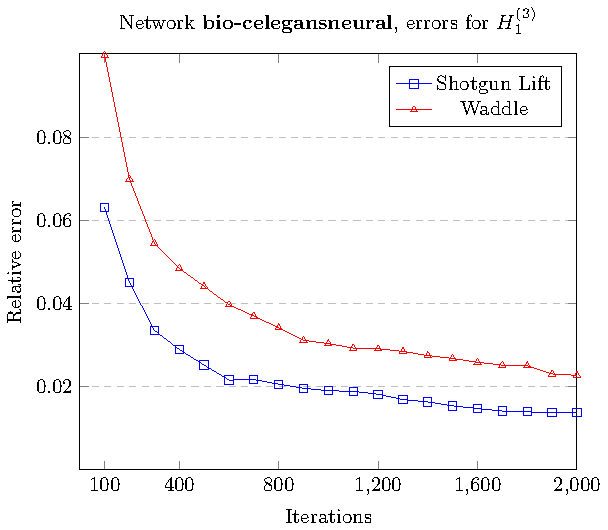
\includegraphics[width=\linewidth]{bio-celegansneural_errors_H_1.pdf}
\endminipage\hfill
\minipage{\myplotwidth}
  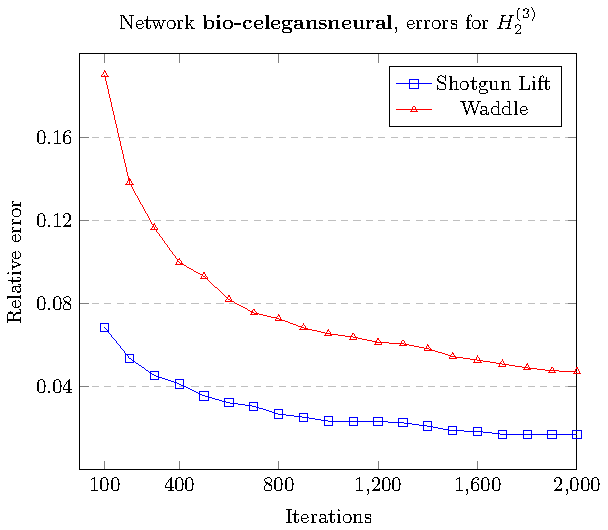
\includegraphics[width=\linewidth]{bio-celegansneural_errors_H_2.pdf}
\endminipage

\hspace*{\fill}
\vskip 1pt
\hspace*{\fill}

\minipage{\myplotwidth}%
  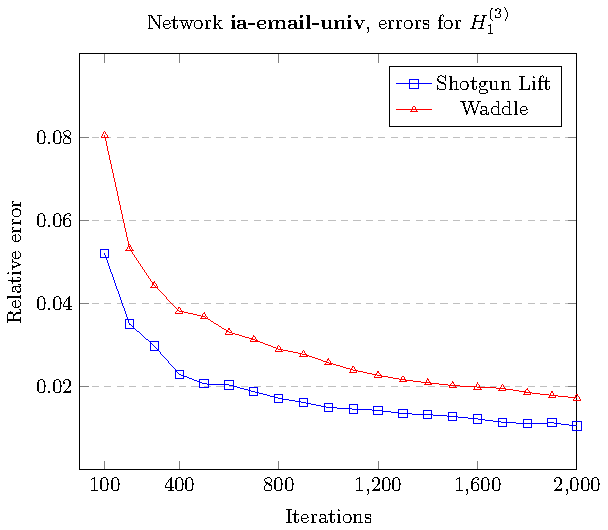
\includegraphics[width=\linewidth]{ia-email-univ_errors_H_1.pdf}
\endminipage\hfill
\minipage{\myplotwidth}
  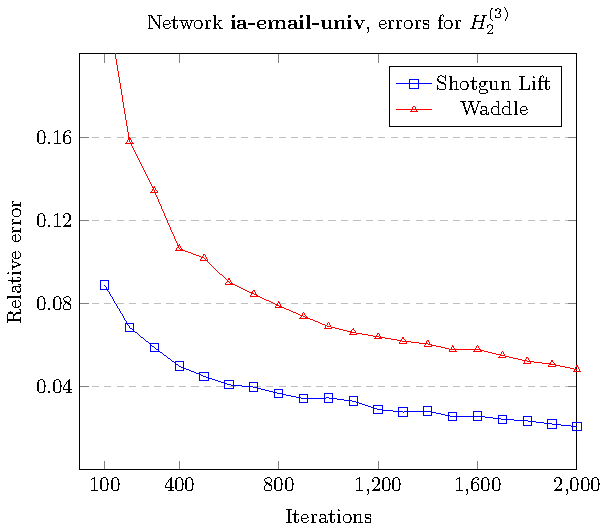
\includegraphics[width=\linewidth]{ia-email-univ_errors_H_2.pdf}
\endminipage

\hspace*{\fill}
\vskip 1pt
\hspace*{\fill}

\minipage{\myplotwidth}%
  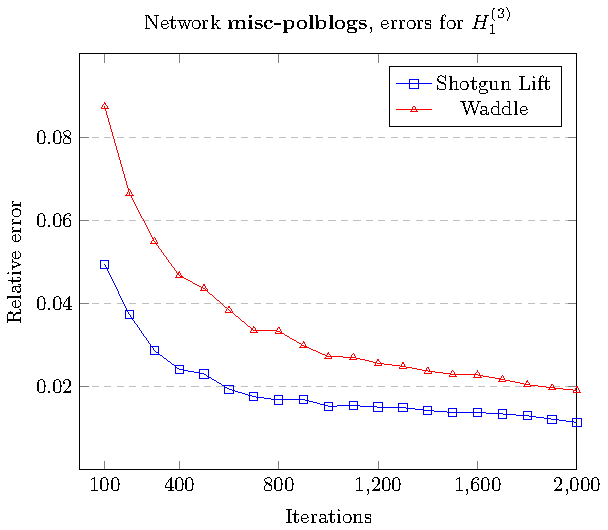
\includegraphics[width=\linewidth]{misc-polblogs_errors_H_1.pdf}
\endminipage\hfill
\minipage{\myplotwidth}
  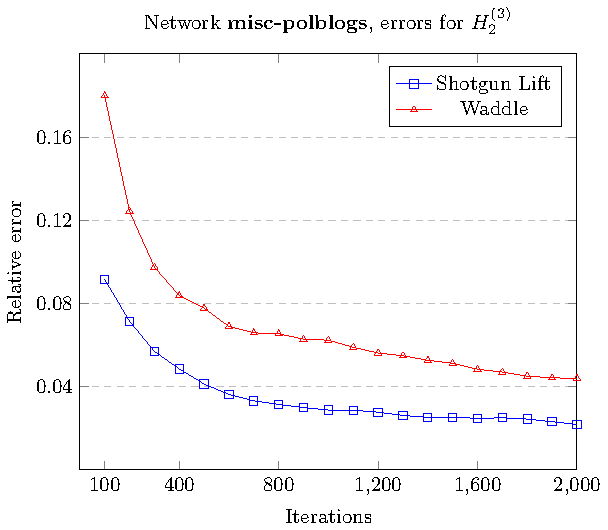
\includegraphics[width=\linewidth]{misc-polblogs_errors_H_2.pdf}
\endminipage

\hspace*{\fill}
\vskip 1pt
\hspace*{\fill}

\minipage{\myplotwidth}%
  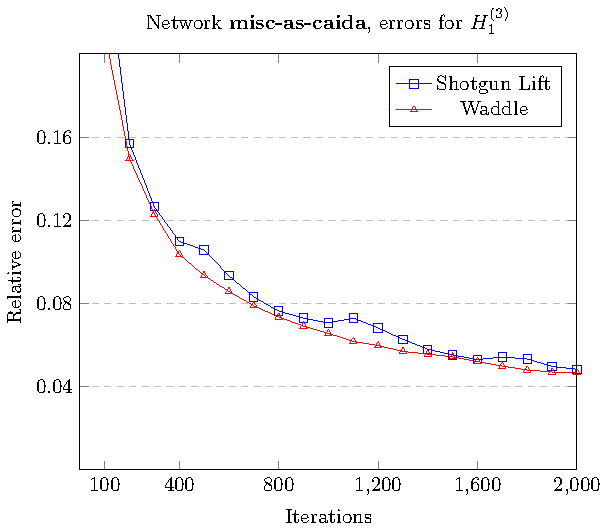
\includegraphics[width=\linewidth]{misc-as-caida_errors_H_1.pdf}
\endminipage\hfill
\minipage{\myplotwidth}
  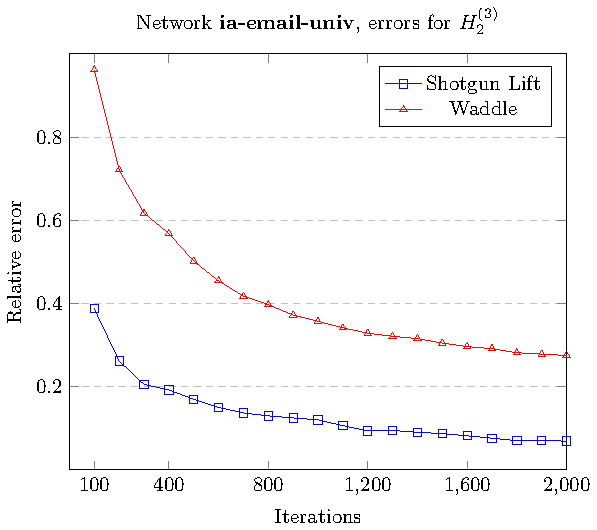
\includegraphics[width=\linewidth]{misc-as-caida_errors_H_2.pdf}
\endminipage

\hspace*{\fill}
\vskip 1pt
\hspace*{\fill}

\minipage{\myplotwidth}%
  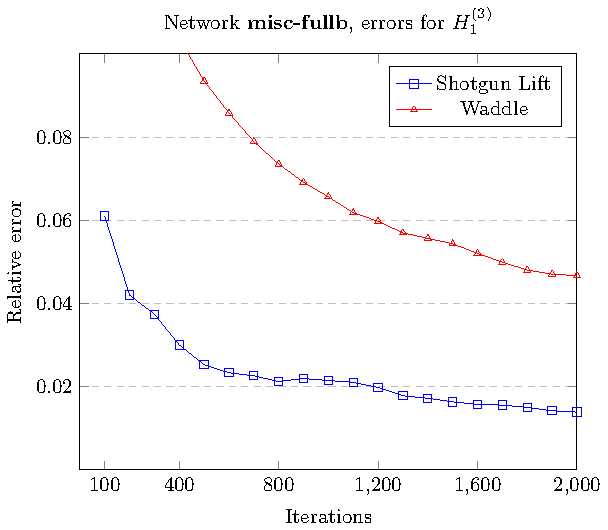
\includegraphics[width=\linewidth]{misc-fullb_errors_H_1.pdf}
\endminipage\hfill
\minipage{\myplotwidth}
  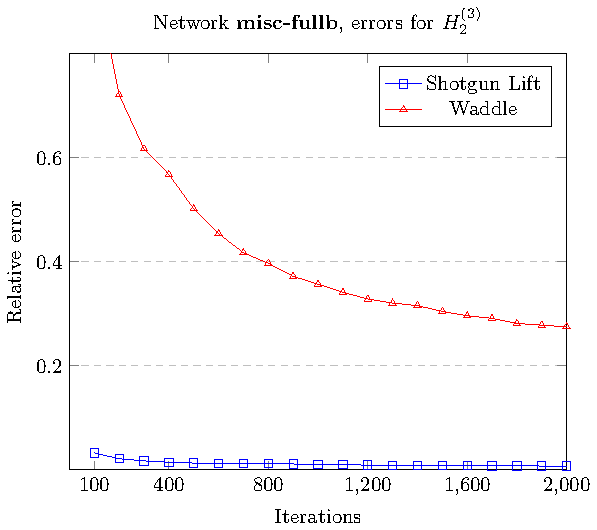
\includegraphics[width=\linewidth]{misc-fullb_errors_H_2.pdf}
\endminipage
\hspace*{\fill}
\end{center}
\caption{Relative errors of count estimators for $H_1^{(3)}$ and $H_2^{(3)}$.}
\label{fig:relative_errors}
\end{figure}

\begin{figure}[th!]
\begin{center}

\minipage{\myplotwidth}
  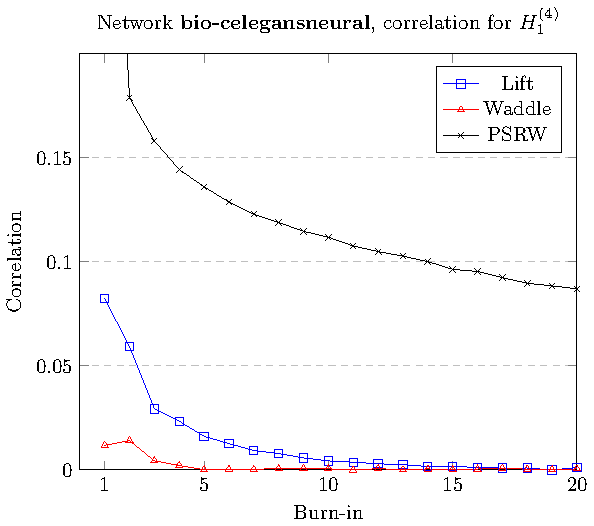
\includegraphics[width=\linewidth]{bio-celegansneural_H_1.pdf}
\endminipage\hfill
\minipage{\myplotwidth}
  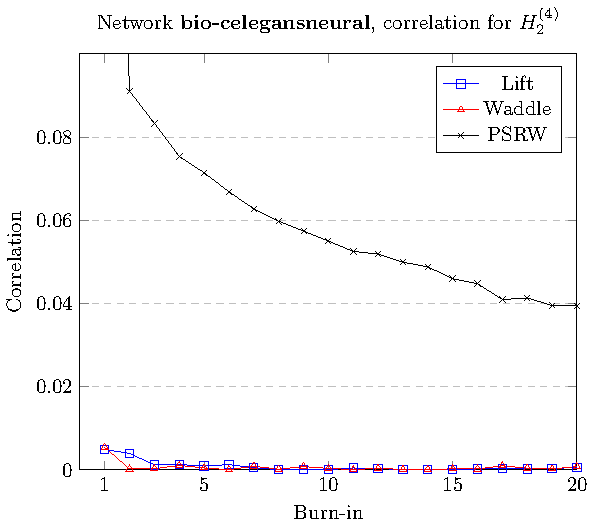
\includegraphics[width=\linewidth]{bio-celegansneural_H_2.pdf}
\endminipage

\hspace*{\fill}
\vskip 1pt
\hspace*{\fill}

\minipage{\myplotwidth}%
  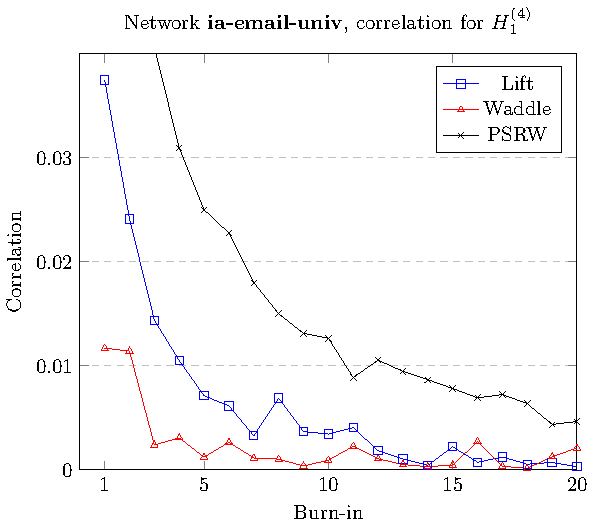
\includegraphics[width=\linewidth]{ia-email-univ_H_1.pdf}
\endminipage\hfill
\minipage{\myplotwidth}
  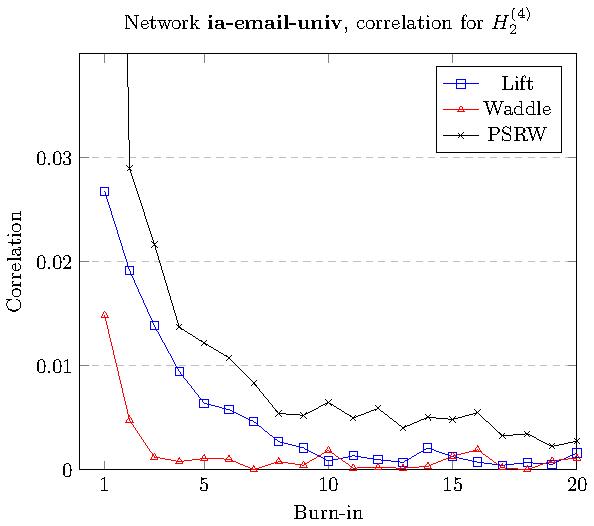
\includegraphics[width=\linewidth]{ia-email-univ_H_2.pdf}
\endminipage

\hspace*{\fill}
\vskip 1pt
\hspace*{\fill}

\minipage{\myplotwidth}%
  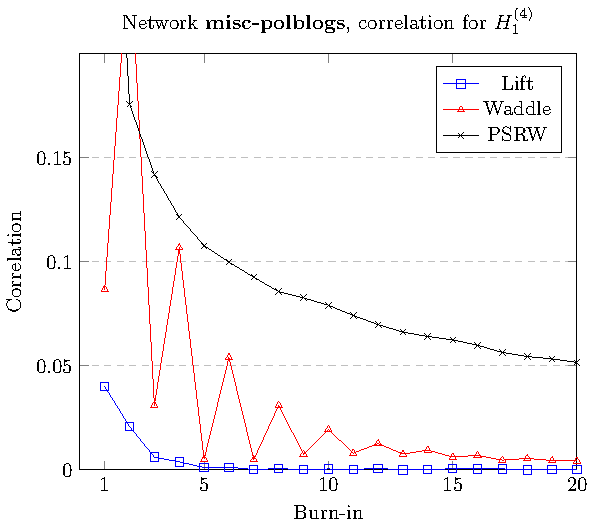
\includegraphics[width=\linewidth]{misc-polblogs_H_1.pdf}
\endminipage\hfill
\minipage{\myplotwidth}
  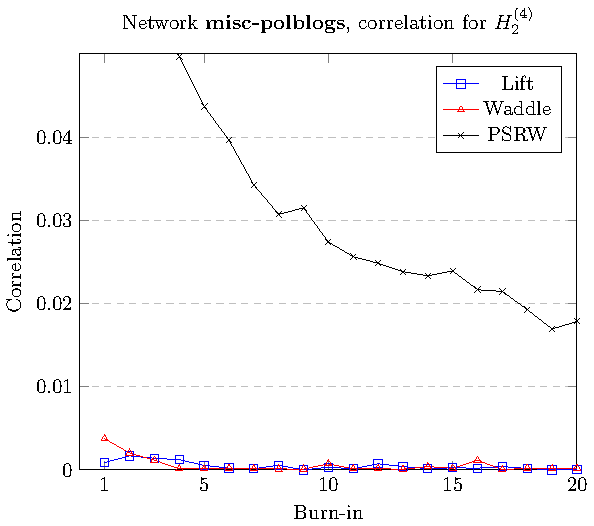
\includegraphics[width=\linewidth]{misc-polblogs_H_2.pdf}
\endminipage

\hspace*{\fill}
\vskip 1pt
\hspace*{\fill}

\minipage{\myplotwidth}%
  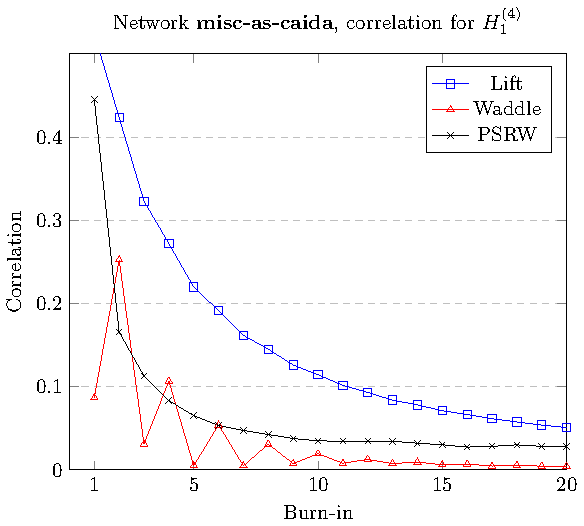
\includegraphics[width=\linewidth]{misc-as-caida_H_1.pdf}
\endminipage\hfill
\minipage{\myplotwidth}
  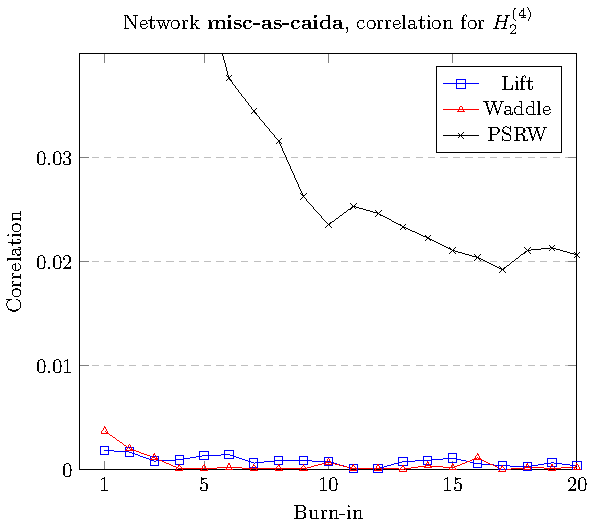
\includegraphics[width=\linewidth]{misc-as-caida_H_2.pdf}
\endminipage

\hspace*{\fill}
\vskip 1pt
\hspace*{\fill}

\minipage{\myplotwidth}%
  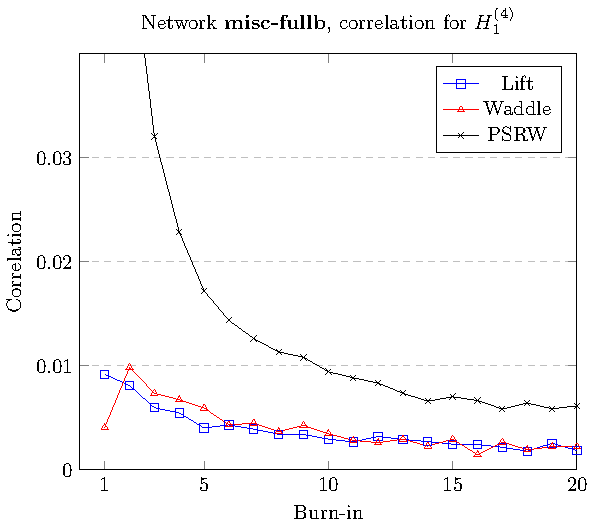
\includegraphics[width=\linewidth]{misc-fullb_H_1.pdf}
\endminipage\hfill
\minipage{\myplotwidth}
  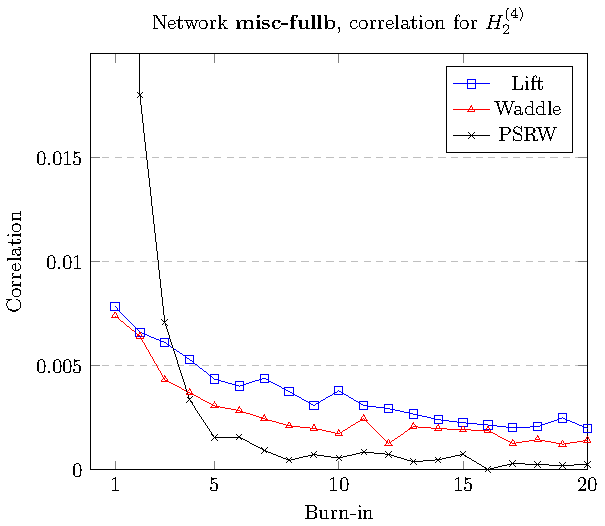
\includegraphics[width=\linewidth]{misc-fullb_H_2.pdf}
\endminipage

\hspace*{\fill}
\end{center}
\caption{Correlation of $\phi_i$ and $\phi_{i+1}$ depending on the intermediate burn-in time, $h$, between samples for graphlets $H_1^{(4)}$ and $H_2^{(4)}$.}
\label{fig:correlation}
\end{figure}

%\subsection{Implementation details}

We demonstrate performance of the shotgun and unordered lift method compared to two competitive methods: PSRW and Waddling.
All algorithms were implemented in Python, and the code is available on GitHub\footnote{github.com/KirillP23/LiftSRW}.

We will compare the effectiveness of estimators in two ways:
\begin{enumerate}
\item Relative error of a graphlet count estimator with $k=3$ (wedges $H_1^{(3)}$ and triangles $H_2^{(3)}$) given limited number of queries (or, equivalently, limited number of samples).
\item Variance and correlation of samples for a graphlet count estimator for 3-stars $H_1^{(4)}$ and 4-paths $H_2^{(4)}$.
\end{enumerate}

In all methods, the first vertex of the lifting procedure is taken from a standard random walk on vertices.
Whenever we specify the burn-in, that would correspond to the random walk steps taken to sample the starting vertex in case of Lifting and Waddling, and the number of steps taken between sampling CISs in case of PSRW.
We compare the Shotgun Lift estimator against Waddling estimator for the first problem, and compare the Unordered Lift estimator against PSRW and Waddling for the second problem.

\subsection{Relative Error given limited queries}

The brute force method gives us the exact graphlet count for $k=3$:

\begin{table}[th]
    \centering
    \begin{tabular}{|l|r|r|}
    \hline
    \multicolumn{3}{ |c| }{Graphlet counts for $k=3$}\\
    \hline
    Network name & $H_1^{(3)}$ & $H_2^{(3)}$  \\
    \hline
    \textbf{bio-celegansneural} & 4.408E+04 & 3.241E+03 \\
    \textbf{ia-email-univ} & 8.038E+04 & 5.343E+03	\\
    \textbf{misc-polblogs} & 1.038E+06 & 1.010E+05	\\	
    \textbf{misc-as-caida} & 1.479E+07 & 3.636E+04 \\
    \textbf{misc-fullb} & 1.620E+08 & 6.021E+07 \\
    \hline
    \end{tabular}
\end{table}

We will compare the relative error 
\begin{equation*}
    \text{relative error} = \frac{|\hat N_m(G) - N_m(G)|}{N_m(G)}
\end{equation*}
between Shotgun Lift estimator and Waddling estimator with burn-in $3$. The number of queries required for each sample $B\in V_G^{(2)}$ is $4$ for the Shotgun Lift algorithm and the number of queries for each $3$-CIS sample is $5$ for the Waddling algorithm.
We take the average error across $100$ runs.

As we see from the plots in Figure~\ref{fig:relative_errors}, Shotgun Lift method outperforms Waddling by a factor of 2 in most cases.
This agrees with our theory, since the number of actual CISs sampled by the Shotgun method is much bigger than Waddle given the same number of queries.

\subsection{Variation and correlation of samples}

We will use the Unordered Lift estimator, to count all motifs of size $4$, but the performance would be measured in terms of the variance of the estimator, both the "variance under independence" and "covariance" parts.
To get an idea about the distribution of $4$-graphlets, we count the $4$-graphlets with the Unordered Lift estimator.

\begin{table}[th]
    \centering
    \begin{tabular}{|l|r|r|r|}
    \hline
    \multicolumn{4}{ |c| }{Graphlet estimates for $k=4$}\\
    \hline
    Network name & $H_1^{(4)}$ & $H_2^{(4)}$ & $H_3^{(4)}$\\
    \hline
    \textbf{bio-celegansneural} &	6.48E+05 &	5.16E+05 &	1.86E+05 \\
    \textbf{ia-email-univ} &	5.40E+05 &	1.11E+06 & 	2.20E+05 \\
    \textbf{misc-polblogs} &	3.94E+07 & 	3.10E+07 & 	1.58E+07 \\
    \textbf{misc-as-caida} &	7.82E+09 &	2.85E+08 &	4.62E+07 \\
    \textbf{misc-fullb} &	1.07E+09 &	4.83E+09 &	2.71E+09 \\
    \hline
    \end{tabular}
\end{table}

%\begin{table}[th]
%    \centering
%    \begin{tabular}{|l|r|r|r|}
%    \hline
%    \multicolumn{4}{ |c| }{Graphlet estimates for $k=4$}\\
%    \hline
%    Network name & $H_4^{(4)}$ & $H_5^{(4)}$ & $H_6^{(4)}$\\
%    \hline
%    \textbf{bio-celegansneural} & 	1.66E+04 &	2.26E+04 & 	2.03E+03 %\\
%    \textbf{ia-email-univ} &	1.24E+04 &	2.04E+04 & 	3.46E+03 \\
%    \textbf{misc-polblogs} &	1.16E+06 &	2.82E+06 &	4.37E+05 \\
%    \textbf{misc-as-caida} &	4.08E+05 &	1.60E+06 &	4.44E+04 \\
%    \textbf{misc-fullb} &	6.43E+07 &	8.95E+08 &	3.71E+08 \\
%    \hline
%    \end{tabular}
%\end{table}

Denote $\phi_i = \frac{\ind(T_i\sim H_m)}{\pi(T_i)}$ for all estimators.
%Waddling, PSRW and Unordered Lift estimators.
Note that $\E \phi_1 = N_m(G)$.
We compare the variance of the estimator $\hat N_m$ using equation \eqref{eq:variance}.
The table below shows estimates for $V_m^{\independent}(\phi_1)$:

\begin{table}[th]
    \centering
    \begin{tabular}{ |l|c||r|r|r| }
    \hline
    \multicolumn{5}{ |c| }{Variation under independence} \\
    \hline
    Network Name & ID & Lift & Waddle & PSRW \\ 
    \hline
    \multirow{2}{*}{\textbf{bio-celegansneural}}
    % & $H_1^{(3)}$ & 0.740 &	1.716 &	0.219 \\
    % & $H_2^{(3)}$ & 5.061 &	6.264 &	4.553 \\
    & $H_1^{(4)}$ & 6.876 &	11.064 &	0.652 \\
    & $H_2^{(4)}$ & 5.470 &	3.956 &	5.185 \\
    \hline
    \multirow{2}{*}{\textbf{ia-email-univ}}
    % & $H_1^{(3)}$ & 0.465 &	0.916 &	0.197 \\
    % & $H_2^{(3)}$ & 6.193 &	6.885 &	5.052 \\
    & $H_1^{(4)}$ & 5.266 &	4.164 &	1.179 \\
    & $H_2^{(4)}$ & 3.272 &	2.958 &	2.216 \\
    \hline
    \multirow{2}{*}{\textbf{misc-polblogs}}
    % & $H_1^{(3)}$ & 0.614 &	1.452 &	0.287 \\
    % & $H_2^{(3)}$ & 4.368 &	4.951 &	3.483 \\
    & $H_1^{(4)}$ & 5.033 &	7.210 &	0.820 \\
    & $H_2^{(4)}$ & 6.214 &	5.369 &	6.093 \\
    \hline
    \multirow{2}{*}{\textbf{misc-as-caida}}
    % & $H_1^{(3)}$ & 1.895 &	4.731 &	0.006 \\
    % & $H_2^{(3)}$ & 176.0 &	246.1 &	165.3 \\
    & $H_1^{(4)}$ & 4.076 &	9.028 &	0.019 \\
    & $H_2^{(4)}$ & 106.06 &	153.11 &	78.87 \\
    \hline
    \multirow{2}{*}{\textbf{misc-fullb}}
    % & $H_1^{(3)}$ & 1.205 &	1.361 & 1.105\\
    % & $H_2^{(3)}$ & 0.911 & 0.957 & 0.904\\
    & $H_1^{(4)}$ & 21.617 &	10.185 &	6.179\\
    & $H_2^{(4)}$ & 6.014 &	4.041 & 3.785\\
    \hline
    \end{tabular}
\end{table}

We can see that PSRW generally has smaller variation under independence, mostly because of the probability $\pi(T)$ being independent of the degrees of vertices of $T$.
On the other hand, variation under independence of Lift and Waddle methods is comparable, meaning that $\pi(T)$ varies similarly for those two methods. 
Next, we compare the dependence of $\phi_i$ and $\phi_{i+1}$ using correlation for different values of the burn-in $h$ (see Fig.\ref{fig:correlation}).
For Lift and Waddling, the burn-in between $\phi_i$ and $\phi_{i+1}$ is the number of steps taken after sampling $T_i$ to get a new starting vertex for $T_{i+1}$.
For PSRW, burn-in is the number of steps between CIS samples in the random walk on subgraphs.
From the graphs in Figure~\ref{fig:correlation}, we see that PSRW produces highly correlated samples compared to Lift and Waddling methods.
This agrees with our analysis of PSRW, since it takes many more steps for the subgraph random walk to achieve desired mixing compared to the random walk on vertices.

\section{Conclusion}
We introduced a flexible methodology for sampling graphlets, called Lifting.
Our experimental results demonstrate our hypothesis that lifting can have smaller variance than Waddling, and better mixing rates than Subgraph Random Walking.
This was reinforced by our theoretical results that control the variance of and covariance between graphlet updates.
We anticipate that this lifting scheme will have more far reaching implications, as we may apply graphlet sampling to supervised learning over graphs and other machine learning applications. 

~\newline
%\section{Conclusion}
\noindent
{\bf Acknowledgements:} JS is supported by NSF DMS-1712996.
%\subsection*{Acknowledgments}

%Grant support, people that helped.


% Then
% \begin{multline*}
%     \frac{2}{n^2} \left\vert\sum_{i < j} \Cov_{\pi_k}\left(\phi(T_i), \phi(T_j)\right) \right\vert \leq\\
%     \frac{16}{n} N_m(G)|E_G|^2 D \sum_{h=1}^\infty \gamma_X(h\tau) \leq \\
%     \frac{16}{n} N_m(G)|E_G|^2 D \frac{e^{-(1-\mu)\tau}}{1-e^{-(1-\mu)\tau}}.
% \end{multline*}

% \subsection{Mixing Time}
% In order to assess the mixing time of the we will use the concept of $\beta$-mixing.
% \begin{definition}
%   The $\beta$-mixing coefficient of a Markov chain with discrete state space, $X_t \in \mathcal X$, is
%   \begin{multline*}
%     \beta_X(t,h) :=\\
%     \sum_{x_0,x_1 \in \mathcal X} |\mathbb P\{ X_t = x_0, X_{t+h} = x_1\} - \mathbb P\{ X_t = x_0 \} \mathbb P\{ X_{t+h} = x_1 \} |.
%   \end{multline*}
% \end{definition}

% \begin{theorem}
%   Let $X_t$ be the random walk over the graph $G$ and let $Y_{t}$ be the graphlet extracted from the $k$-lifting process.
%   Then
%   \begin{equation}
%     \mathbb \beta_X(t,h) \ge \mathbb \beta_Y(t,h).
%   \end{equation}
% \end{theorem}

% \begin{proof}
%   Let $Q_1 ( x_t, x_{t+h} ) = \mathbb P \{ X_t = x_t, X_{t+h} = x_{t+h} \}$ and $Q_2 = \mathbb P \{ X_t = x_t\} \mathbb P\{X_{t+h} = x_{t+h}\}$.
%   Also, let $P_1, P_2$ be the joint distributions of $Y_t, Y_{t+h}$ when $X_t, X_{t+h}$ are drawn according to $Q_1,Q_2$ respectively.
%   Due to the lifting process, the distribution of $Y_t, Y_{t+h} | X_t, X_{t+h}$ is invariant to the choice of distribution of $X_t, X_{t+h}$ (being from $Q_1$ or $Q_2$).
%   Hence, by the generalized data processing inequality we have that
%   \begin{equation*}
%     D_f(Q_1 || Q_2) \ge D_f(P_1 || P_2),
%   \end{equation*}
%   for any $f$-divergence.
%   By selecting the total variation divergence, we have the result.
% \end{proof}

